%%%%%%%%%%%%%%%%%%%%%%%%%%%%%%%%%%%%%%%%%%%%%%%%%%%%%%%%%%%%%%%%%%%%%%%%%%%%%%%%%%%
%% This project aims to create the UFC template for presentation.                %%
%% author: Maurício Moreira Neto - Doctoral student in Computer Science (MDCC)   %%
%% contacts:                                                                     %%
%%    e-mail: maumneto@ufc.br                                                    %%
%%    linktree: https://linktr.ee/maumneto                                       %%
%%%%%%%%%%%%%%%%%%%%%%%%%%%%%%%%%%%%%%%%%%%%%%%%%%%%%%%%%%%%%%%%%%%%%%%%%%%%%%%%%%%
\documentclass{libs/ufc_format}
% Inserting the preamble file with the packages
\input{libs/preamble.tex}
% Inserting the references file
\bibliography{references.bib}

% Title
\title[Previsão do preço do ouro]{\huge\textbf{Previsão multi-horizonte do preço do ouro:}\\\Large\textbf{uma comparação entre modelos lineares, \emph{boosting} e redes neurais profundas sobre log-retornos}}
% Author of the presentation
\author[]{Francisco Paulino Arruda Filho \\ Ivina Lorena Oliveira Moura \\ Gabriel de Souza Mendes \\ José Vinícius Evangelista Dias de Souza}
% Institute's Name
\institute[UFC]{
    % email for contact
    \small{\email{\{paulinofilho, ivinalorena, gabrielmendes01, joseedsouza\}@alu.ufc.br}}
}
% date of the presentation
\date[]{}


%%%%%%%%%%%%%%%%%%%%%%%%%%%%%%%%%%%%%%%%%%%%%%%%%%%%%%%%%%%%%%%%%%%%%%%%%%%%%%%%%%
%% Start Document of the Presentation                                           %%               
%%%%%%%%%%%%%%%%%%%%%%%%%%%%%%%%%%%%%%%%%%%%%%%%%%%%%%%%%%%%%%%%%%%%%%%%%%%%%%%%%%
\begin{document}
% insert the code style
\input{libs/code_style}

%% ---------------------------------------------------------------------------
% First frame (with tile, subtitle, ...)
{
\usebackgroundtemplate{
\includegraphics[width=1.7\paperwidth]{libs/logoUFCbackground.png}}
\logo{\hspace*{-1.6cm}
\includegraphics[scale=0.075]{libs/emblemufc.pdf}\hspace{9.7cm} \vspace{-0.2cm}}
\begin{frame}{}
    \maketitle
\end{frame}
}
\usebackgroundtemplate{}

%% ---------------------------------------------------------------------------
% Second frame
\begin{frame}{Sumário}
    \begin{columns}[t]
        \begin{column}{0.48\textwidth}
            \tableofcontents[hidesubsections,sections={1-3}]
        \end{column}
        \begin{column}{0.48\textwidth}
            \tableofcontents[hidesubsections,sections={4-6}]
        \end{column}
    \end{columns}
\end{frame}

%% ---------------------------------------------------------------------------
\section{Motivação}
\subsection{O Problema}

\begin{frame}{Por que o ouro é difícil de prever?}
    \begin{itemize}
        \item O ouro funciona como \emph{ativo de reserva} e \emph{hedge}: reage a inflação, crises geopolíticas, juros reais e força do dólar.
        \item Isso torna a dinâmica do preço sensível a \emph{choques macroeconômicos} e mudanças de regime.
        \item Em horizontes curtos, o sinal preditível é \emph{fraco} e fica imerso em ruído de mercado.
        \item Mesmo quando existe algum padrão, ele tende a ser \emph{marginal} e instável ao longo do tempo.
    \end{itemize}

    \vspace{0.3cm}
    \alertbox{\textbf{Tensão central do trabalho:} pode existir sinal útil, mas ele é pequeno o bastante para ser facilmente confundido com acaso ou vazamento de informação.}
\end{frame}

%% ---------------------------------------------------------------------------
\begin{frame}{Não-estacionariedade e extrapolação}
    \begin{itemize}
        \item O preço saiu de cerca de \textbf{US\$ 280/onça} em 2000 para mais de \textbf{US\$ 3000/onça} em 2025.
        \item O nível da série muda demais ao longo do tempo: a média não é estável.
        \item Um modelo treinado no \emph{preço bruto} não vê, no treino, os mesmos patamares que aparecem no teste.
        \item Isso vira um problema de \emph{extrapolação}, não apenas de previsão.
    \end{itemize}
\end{frame}

%% ---------------------------------------------------------------------------
\begin{frame}{Preço diário do ouro (2000--2025)}
    \begin{figure}
        \centering
        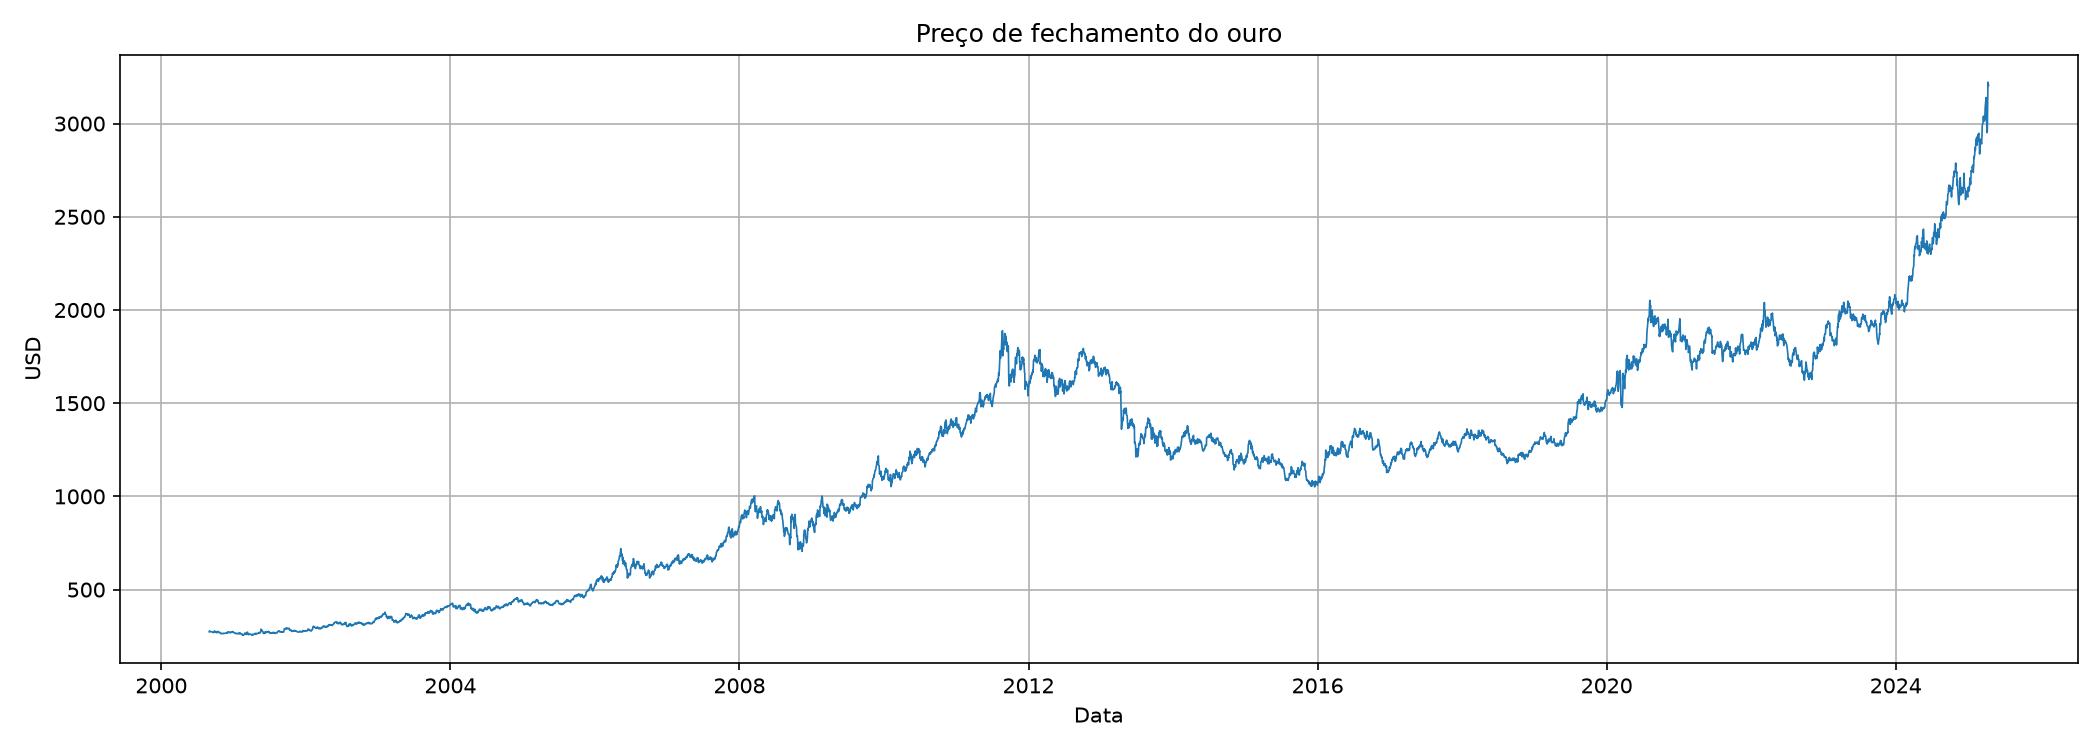
\includegraphics[width=0.92\linewidth]{figs/serie_preco.png}
        \caption{Preço de fechamento diário do ouro entre 2000 e 2025.}
    \end{figure}
\end{frame}

%% ---------------------------------------------------------------------------
\begin{frame}{Mercado eficiente e \emph{random walk}}
    \begin{block}{Ponto de partida}
        Se os mercados incorporam rapidamente a informação disponível, o melhor palpite para o preço de amanhã é o preço de hoje \cite{fama1970efficient}.
    \end{block}

    \vspace{0.2cm}

    \begin{itemize}
        \item Esse é o raciocínio do \emph{random walk}: mudanças de curto prazo são próximas de imprevisíveis.
        \item A série pode ter memória de regimes e tendência em horizontes maiores, mas o ruído domina no dia a dia.
        \item Por isso, bater um \emph{baseline} ingênuo já é um critério forte de qualidade.
    \end{itemize}

    \vspace{0.3cm}
    \successbox{O desafio não é só prever bem; é demonstrar que o ganho é real e não ilusão estatística.}
\end{frame}

%% ---------------------------------------------------------------------------
\subsection{Primeira Tentativa}

\begin{frame}{Nossa primeira tentativa (que falhou)}
    \begin{itemize}
        \item A hipótese inicial era simples: \emph{se enriquecermos bem os dados, um bom modelo aprende o preço do ouro}.
        \item Em um experimento anterior (2025), foi usada \emph{Ridge Regression} para prever o preço \textbf{1 dia à frente}.
        \item O código desse experimento ficou disponível em:
    \end{itemize}

    \vspace{0.2cm}
    \simplebox{\scriptsize \url{https://github.com/JoseEdSouza/machine-learning-works/blob/main/gold/eda.ipynb}}

    \vspace{0.3cm}
    \alertbox{\textbf{Moral inicial:} o problema parecia ser ``escolher um modelo melhor'', mas a falha principal estava na formulação e no protocolo.}
\end{frame}

%% ---------------------------------------------------------------------------
\begin{frame}{Onde o experimento anterior errou}
    \begin{itemize}
        \item Antes do \emph{split}, as amostras foram embaralhadas com \emph{shuffle} aleatório.
        \item Isso mistura observações do passado e do futuro entre treino e teste.
        \item Em séries temporais, esse procedimento gera \textbf{vazamento temporal}.
        \item O modelo parece aprender muito bem, mas parte desse desempenho vem de uma avaliação contaminada.
        \item Resultado: \emph{overfitting} otimista e uma noção falsa de generalização.
    \end{itemize}

    \vspace{0.3cm}
    \begin{block}{Conclusão}
        O erro central não era só o modelo. Era tentar prever o \emph{preço bruto} sob um protocolo de avaliação quebrado.
    \end{block}
\end{frame}

%% ---------------------------------------------------------------------------
\section{Dados e Reformulação}
\subsection{Os Dados}

\begin{frame}{Os dados}
    \begin{itemize}
        \item \textbf{Fonte:} \emph{Precious Metals History since 2000 with News}, disponível no Kaggle \cite{kaggle_precious_metals}.
        \item \textbf{Período:} 2000--2025, com frequência diária.
        \item \textbf{Colunas principais:} OHLC (\emph{open, high, low, close}), volume e \emph{headlines}.
        \item A coluna \emph{headlines} reúne, para cada pregão, manchetes associadas àquela data, vindas de diferentes jornais/fontes noticiosas.
        \item \textbf{Alvo:} log-retorno acumulado para $h \in \{5, 15, 30\}$ pregões.
        \item O problema deixa de ser prever nível de preço e passa a ser prever variação futura acumulada.
    \end{itemize}
\end{frame}

%% ---------------------------------------------------------------------------
{\logo{}
\begin{frame}{Como construímos a feature textual}
    \begin{itemize}
        \item Se a coluna \texttt{headlines} existe, o texto é convertido para minúsculas e valores ausentes viram string vazia.
        \item Em seguida, contamos ocorrências de um léxico de termos de estresse:
        \item \scriptsize \texttt{crisis, crash, war, recession, inflation, default, collapse, panic, fear, conflict, sanction, bankrupt, plunge, turmoil, slump, selloff, attack, invasion, pandemic, virus}
        \normalsize
        \item O índice principal é:
        \[
            \texttt{fear\_ratio}
            =
            \frac{\#\text{termos do léxico}}{\#\text{separadores "/" nas manchetes} + 1}
        \]
        \item Depois calculamos \texttt{fear\_ma5}, uma média móvel de 5 dias desse índice.
    \end{itemize}

    \vspace{0.2cm}
    \simplebox{\textbf{Intuição:} quanto mais palavras associadas a crise e pânico aparecem nas manchetes do pregão, maior o sinal textual de medo.}
\end{frame}
}

%% ---------------------------------------------------------------------------
{\logo{}
\begin{frame}{Atributos de entrada ($d=19$)}
    \scriptsize
    \begin{table}
    \centering
    \caption{Atributos de entrada do modelo. Todos são causais e invariantes ao nível de preço.}
    \begin{tabular}{p{0.28\linewidth} p{0.46\linewidth} p{0.16\linewidth}}
        \toprule
        \textbf{Atributo} & \textbf{Definição} & \textbf{Grupo} \\
        \midrule
        \texttt{log\_ret\_1,5,21} & $\log(P_t/P_{t-k}),\; k\in\{1,5,21\}$ & Momentum \\
        \texttt{vol\_5, vol\_21} & desvio-padrão móvel de \texttt{log\_ret\_1} & Volatilidade \\
        \texttt{vol\_ratio} & $\mathrm{vol}_5/\mathrm{vol}_{21}$ ($>1$ = estresse) & Volatilidade \\
        \texttt{dist\_ma20,50} & $P_t/\mathrm{MA}_k - 1,\; k\in\{20,50\}$ & Tendência \\
        \texttt{ma\_cross} & $\mathrm{MA}_{20}/\mathrm{MA}_{50} - 1$ & Tendência \\
        \texttt{rsi} & RSI(14) recentrado em $[-1,1]$ & Oscilador \\
        \texttt{macd\_hist} & histograma MACD normalizado por $P_t$ & Oscilador \\
        \texttt{boll\_b} & posição \%B nas bandas de Bollinger & Oscilador \\
        \texttt{drawdown\_252} & $P_t/\max_{252}(P) - 1$ & Regime \\
        \texttt{hl\_range} & $(\mathrm{high}-\mathrm{low})/P_t$ & Intradiário \\
        \texttt{close\_pos} & posição do fechamento na barra OHLC & Intradiário \\
        \texttt{gap\_open} & $\log(\mathrm{open}_t/P_{t-1})$ & Intradiário \\
        \texttt{volume} & volume negociado no dia & Liquidez \\
        \texttt{fear\_ratio} & índice de medo por léxico nas manchetes & Texto \\
        \texttt{fear\_ma5} & média móvel de 5 dias de \texttt{fear\_ratio} & Texto \\
        \bottomrule
    \end{tabular}
    \end{table}

    \vspace{0.2cm}
    \simplebox{\textbf{Todos os atributos são causais e invariantes ao nível de preço.}}
\end{frame}
}

%% ---------------------------------------------------------------------------
\subsection{Antes da Reformulação}

\begin{frame}{O que tentamos antes de reformular o problema}
    \begin{itemize}
        \item Depois de identificar os erros, treinamos primeiro um \emph{baseline} ingênuo para ter uma referência honesta.
        \item Ficou claro que parte central da dificuldade vinha da inflação empurrando o nível do preço para cima ao longo do tempo.
        \item Também testamos sinais exógenos e textuais para enriquecer os dados antes de mexer no alvo.
        \item A lição foi direta: \emph{enriquecer os dados no espaço errado não resolve o problema estrutural}.
    \end{itemize}

    \vspace{0.3cm}
    \successbox{A virada conceitual do trabalho veio quando deixamos de insistir no preço bruto e passamos a reformular o alvo.}
\end{frame}

%% ---------------------------------------------------------------------------
\begin{frame}{Inflação (CPI)}
    \begin{itemize}
        \item A hipótese era que o CPI ajudaria a explicar a tendência persistente de alta do ouro.
        \item Na prática, a contribuição foi marginal.
        \item Há um problema operacional importante: índices de inflação são calculados e divulgados com atraso.
        \item Se esse atraso não for tratado explicitamente, surge risco de \emph{look-ahead bias} e vazamento temporal.
    \end{itemize}

    \vspace{0.3cm}
    \alertbox{\textbf{Decisão:} descartado. O custo metodológico e o risco de vazamento eram maiores do que o ganho observado.}
\end{frame}

%% ---------------------------------------------------------------------------
\begin{frame}{Petrodólar}
    \begin{itemize}
        \item A hipótese era que ouro e petróleo capturam, em parte, o mesmo estresse geopolítico e macroeconômico.
        \item Em alguns períodos a correlação aparecia, mas ela não era estável ao longo do tempo.
        \item Isso introduziu complexidade extra de alinhamento entre séries e regimes.
        \item O ganho prático foi pequeno demais para justificar a complexidade adicional.
    \end{itemize}

    \vspace{0.3cm}
    \alertbox{\textbf{Decisão:} descartado. Relação plausível economicamente, mas fraca e inconsistente para o protocolo adotado.}
\end{frame}

%% ---------------------------------------------------------------------------
\begin{frame}{Embeddings das manchetes}
    \begin{itemize}
        \item Testamos embeddings \texttt{nomic-embed-text} (\texttt{768} dimensões) como entrada para um XGBoost.
        \item O resultado piorou de forma significativa em relação ao XGBoost baseline.
        \item A interpretação mais provável é combinação de pouco dado útil com alta dimensionalidade.
        \item Embeddings da OpenAI, como \texttt{text-embedding-3-small} e \texttt{text-embedding-3-large}, ficaram no \emph{roadmap}, mas não houve tempo de avaliação adequada.
    \end{itemize}

    \vspace{0.3cm}
    \begin{block}{Leitura correta}
        Não concluímos que texto não ajuda. Concluímos apenas que esse caminho exige mais tempo, melhor representação e experimentação mais cuidadosa.
    \end{block}
\end{frame}

%% ---------------------------------------------------------------------------
\begin{frame}{Moral desse bloco}
    \begin{itemize}
        \item Baseline honesto primeiro.
        \item Variáveis externas mal alinhadas podem criar mais vazamento do que sinal.
        \item Mais atributos n\~ao significam melhor generalização.
        \item O avanço real veio de \textbf{reformular o alvo}, não de empilhar sinais sobre o preço bruto.
    \end{itemize}
\end{frame}

%% ---------------------------------------------------------------------------
\subsection{A Reformulação}

\begin{frame}{A reformulação: parar de prever o preço}
    \begin{itemize}
        \item Em vez de prever o \emph{preço bruto}, passamos a prever o \textbf{log-retorno acumulado}.
        \item Para cada instante $t$, o alvo passa a ser:
    \end{itemize}

    \vspace{0.2cm}
    \begin{equation}
      y_t^{(h)} = \log\!\left(\frac{P_{t+h}}{P_t}\right),
      \qquad h \in \{5, 15, 30\}.
    \end{equation}

    \vspace{0.2cm}
    \begin{itemize}
        \item Ou seja: a pergunta deixa de ser ``qual será o preço futuro?'' e passa a ser ``qual será a variação acumulada nos próximos $5$, $15$ e $30$ pregões?''.
    \end{itemize}

    \vspace{0.3cm}
    \successbox{\textbf{Ideia central:} mudamos a pergunta, não o modelo.}
\end{frame}

%% ---------------------------------------------------------------------------
\begin{frame}{Por que o log-retorno funciona melhor?}
    \begin{itemize}
        \item O log-retorno é \textbf{aproximadamente estacionário} e tende a ficar centrado em zero.
        \item Isso evita o problema de extrapolar para níveis de preço nunca vistos no treino.
        \item Ele também é \textbf{aditivo e simétrico}, o que facilita a modelagem temporal.
        \item Depois da previsão, o preço pode ser reconstruído por:
    \end{itemize}

    \vspace{0.2cm}
    \begin{equation}
      \hat{P}_{t+h} = P_t \cdot \exp\!\big(\hat{y}_t^{(h)}\big).
    \end{equation}

    \vspace{0.2cm}
    \begin{itemize}
        \item Assim, modelamos na escala estatisticamente adequada e avaliamos novamente em US\$/oz.
    \end{itemize}
\end{frame}

%% ---------------------------------------------------------------------------
\begin{frame}{Mudando a pergunta}
    \begin{columns}
        \begin{column}{0.5\textwidth}
            \begin{block}{Antes}
                Prever diretamente o preço bruto de um ativo não-estacionário.
            \end{block}

            \vspace{0.3cm}
            \begin{itemize}
                \item forte tendência
                \item extrapolação difícil
                \item avaliação enganosa
            \end{itemize}
        \end{column}
        \begin{column}{0.5\textwidth}
            \begin{exampleblock}{Depois}
                Prever retornos acumulados em múltiplos horizontes.
            \end{exampleblock}

            \vspace{0.3cm}
            \begin{itemize}
                \item série mais estável
                \item alvo comparável no tempo
                \item avaliação mais honesta
            \end{itemize}
        \end{column}
    \end{columns}
\end{frame}

%% ---------------------------------------------------------------------------
\begin{frame}{Regressão multi-horizonte}
    \begin{itemize}
        \item Cada entrada passa a ser uma janela de \textbf{60 pregões} com atributos causais.
        \item A saída do modelo são \textbf{três previsões simultâneas}: $h=5$, $h=15$ e $h=30$.
        \item Isso enquadra o problema como \textbf{regressão multi-horizonte}.
        \item A arquitetura pode compartilhar representação temporal e aprender padrões úteis para horizontes curtos e longos ao mesmo tempo.
    \end{itemize}

    \vspace{0.3cm}
    \simplebox{Entrada: janela de 60 dias \quad $\longrightarrow$ \quad Saídas: $\{\hat{y}^{(5)}, \hat{y}^{(15)}, \hat{y}^{(30)}\}$}
\end{frame}

%% ---------------------------------------------------------------------------
\section{Protocolo e EDA}
\subsection{Protocolo de Avaliação}

\begin{frame}{Protocolo de avaliação}
    \begin{itemize}
        \item O \emph{split} principal é \textbf{estritamente temporal}: $70\%$ treino, $15\%$ validação e $15\%$ teste.
        \item Não há \emph{shuffle}.
        \item Entre os conjuntos, inserimos um \textbf{gap de 90 pregões} para evitar sobreposição entre janelas e alvos.
        \item Esse gap vem de $L + \max(h) = 60 + 30 = 90$.
    \end{itemize}
\end{frame}

%% ---------------------------------------------------------------------------
\begin{frame}{Divisão temporal com gap anti-vazamento}
    \begin{figure}
        \centering
        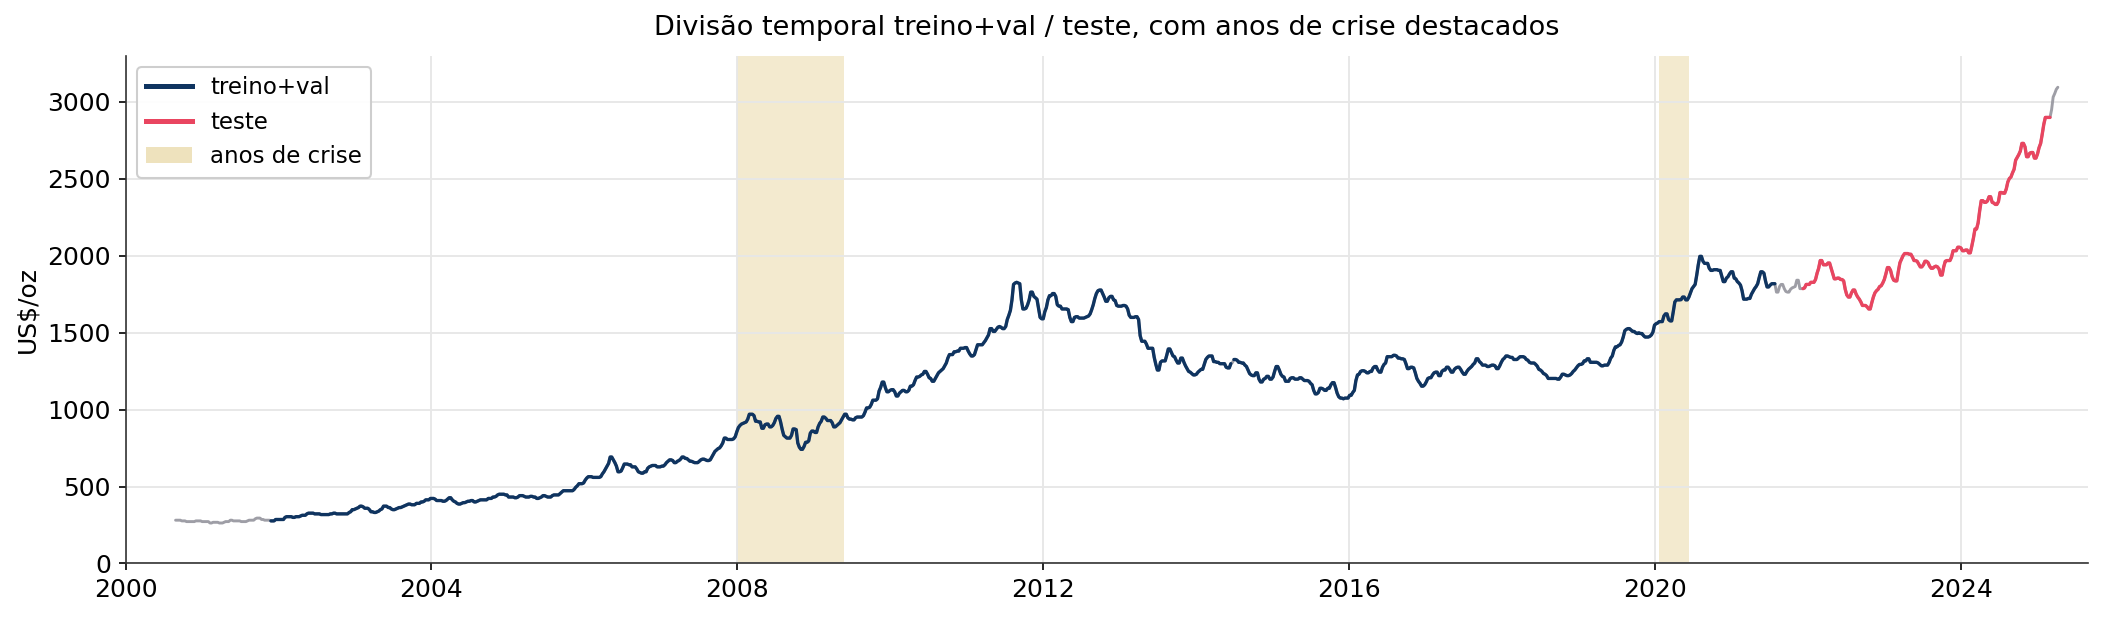
\includegraphics[width=0.98\linewidth]{figs/split_temporal.png}
        \caption{Divisão temporal treino/validação/teste com gap anti-vazamento.}
    \end{figure}
\end{frame}

%% ---------------------------------------------------------------------------
\begin{frame}{Por que esse split é desafiador?}
    \begin{itemize}
        \item A crise de \textbf{2008} fica no treino.
        \item A pandemia de \textbf{2020} aparece na validação.
        \item O forte \emph{rally} de \textbf{2021--2025} fica no teste.
        \item Ou seja: o teste cobra generalização em um regime recente e em patamares de preço muito mais altos.
    \end{itemize}

    \vspace{0.3cm}
    \alertbox{\textbf{Leitura correta:} o protocolo não facilita o problema. Ele força o modelo a enfrentar mudança de regime sem vazamento temporal.}
\end{frame}

%% ---------------------------------------------------------------------------
\begin{frame}{Split único vs. \emph{walk-forward}}
    \begin{columns}
        \begin{column}{0.48\textwidth}
            \begin{block}{Split único}
                \begin{itemize}
                    \item um treino
                    \item uma validação
                    \item um teste final
                \end{itemize}
            \end{block}

            \vspace{0.2cm}
            \small Bom para comparação direta entre modelos.
        \end{column}
        \begin{column}{0.48\textwidth}
            \begin{exampleblock}{Walk-forward}
                \begin{itemize}
                    \item treino expansivo
                    \item folds anuais
                    \item embargo entre treino e teste
                \end{itemize}
            \end{exampleblock}

            \vspace{0.2cm}
            \small Bom para medir robustez em vários regimes.
        \end{column}
    \end{columns}

    \vspace{0.4cm}
    \simplebox{\textbf{Ideia:} o split único responde ``quem foi melhor neste recorte?''; o \emph{walk-forward} responde ``quem sustenta desempenho ao longo do tempo?''}
\end{frame}

%% ---------------------------------------------------------------------------
\begin{frame}{Validação \emph{walk-forward}}
    \begin{itemize}
        \item Depois do \emph{split} principal, usamos validação \emph{walk-forward} como checagem honesta de robustez.
        \item Cada \emph{fold} usa \textbf{treino expansivo} e um bloco de teste de aproximadamente \textbf{252 pregões} (cerca de 1 ano).
        \item Entre treino e teste, há \textbf{embargo} para impedir contaminação temporal.
        \item Isso produz uma distribuição de desempenho ao longo de anos e regimes diferentes, em vez de um único número.
    \end{itemize}
\end{frame}

%% ---------------------------------------------------------------------------
\subsection{EDA}

\begin{frame}{EDA: confirmando que o problema é duro}
    \begin{itemize}
        \item A análise exploratória foi usada para testar se a série trazia sinal estatístico simples ou apenas ruído.
        \item O resultado foi consistente com a dificuldade esperada para séries financeiras.
        \item Os log-retornos exibem caudas pesadas, pouca autocorrelação linear e forte agrupamento de volatilidade.
        \item Em outras palavras: há estrutura, mas ela não é fácil de capturar com modelos ingênuos.
    \end{itemize}
\end{frame}

%% ---------------------------------------------------------------------------
\begin{frame}{Distribuição dos log-retornos}
    \begin{figure}
        \centering
        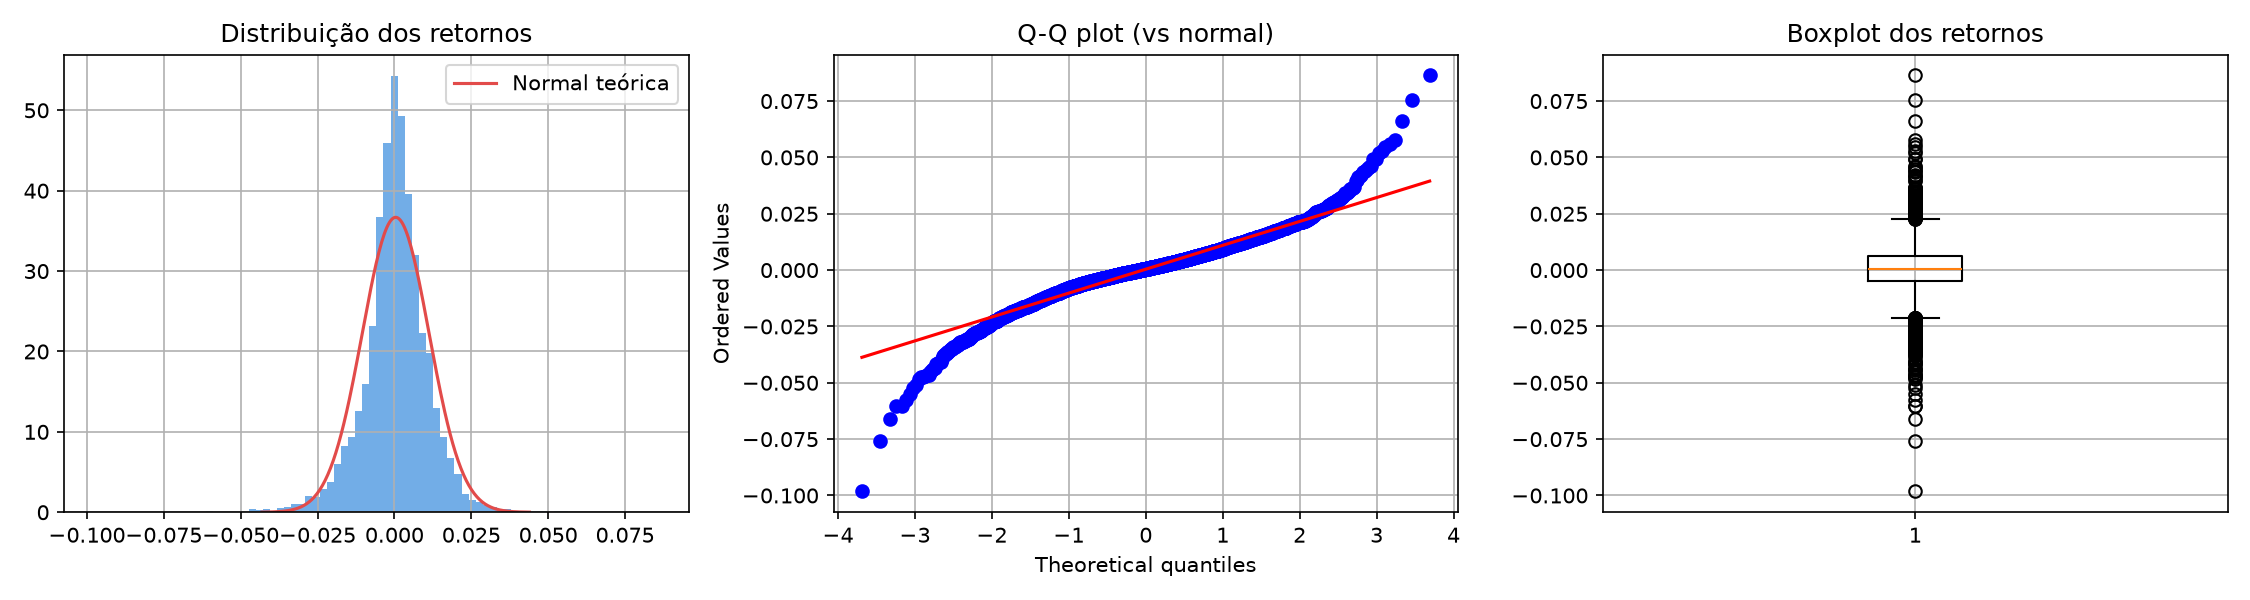
\includegraphics[width=0.94\linewidth]{figs/distribuicao_retornos.png}
        \caption{Histograma, Q-Q plot e boxplot dos log-retornos diários do ouro.}
    \end{figure}

    \vspace{0.2cm}
    \simplebox{Os log-retornos são \textbf{leptocúrticos}, com \textbf{caudas pesadas} e \textbf{assimetria negativa}.}
\end{frame}

%% ---------------------------------------------------------------------------
\begin{frame}{ADF: preço vs. log-retorno}
    \centering
    \begin{tabular}{p{0.34\linewidth} p{0.24\linewidth} p{0.28\linewidth}}
        \toprule
        \textbf{Série} & \textbf{Resultado ADF} & \textbf{Interpretação} \\
        \midrule
        Preço do ouro & não rejeita raiz unitária & não-estacionária \\
        Log-retorno diário & rejeita raiz unitária & aproximadamente estacionária \\
        \bottomrule
    \end{tabular}

    \vspace{0.4cm}
    \alertbox{A evidência estatística reforça a decisão de modelar \textbf{retornos}, e não o \textbf{preço bruto}.}
\end{frame}

%% ---------------------------------------------------------------------------
{\logo{}
\begin{frame}{ACF e PACF dos log-retornos}
    \begin{figure}
        \centering
        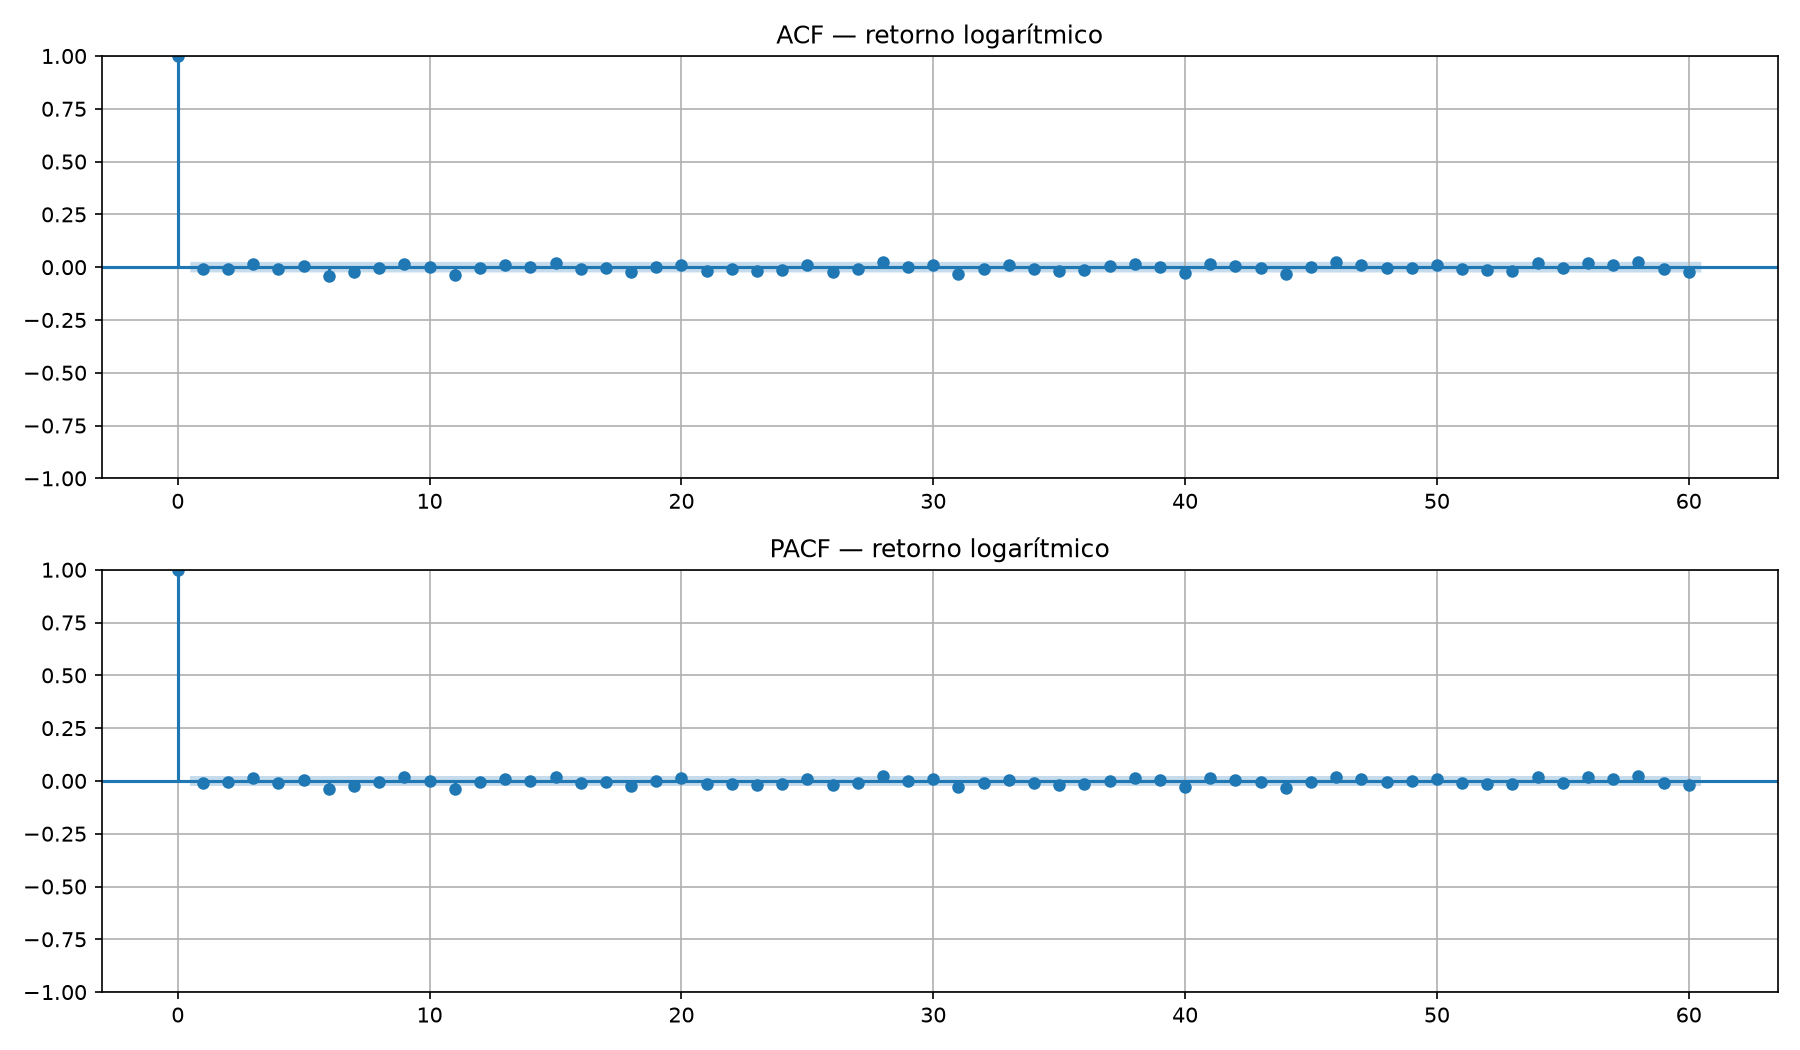
\includegraphics[width=0.82\linewidth]{figs/acf_pacf.png}
        \caption{ACF e PACF dos log-retornos do ouro.}
    \end{figure}

    \vspace{0.2cm}
    \simplebox{A autocorrelação linear é \textbf{fraca} e, em grande parte, \textbf{não significativa}.}
\end{frame}
}

%% ---------------------------------------------------------------------------
\begin{frame}{Volatility clustering}
    \begin{figure}
        \centering
        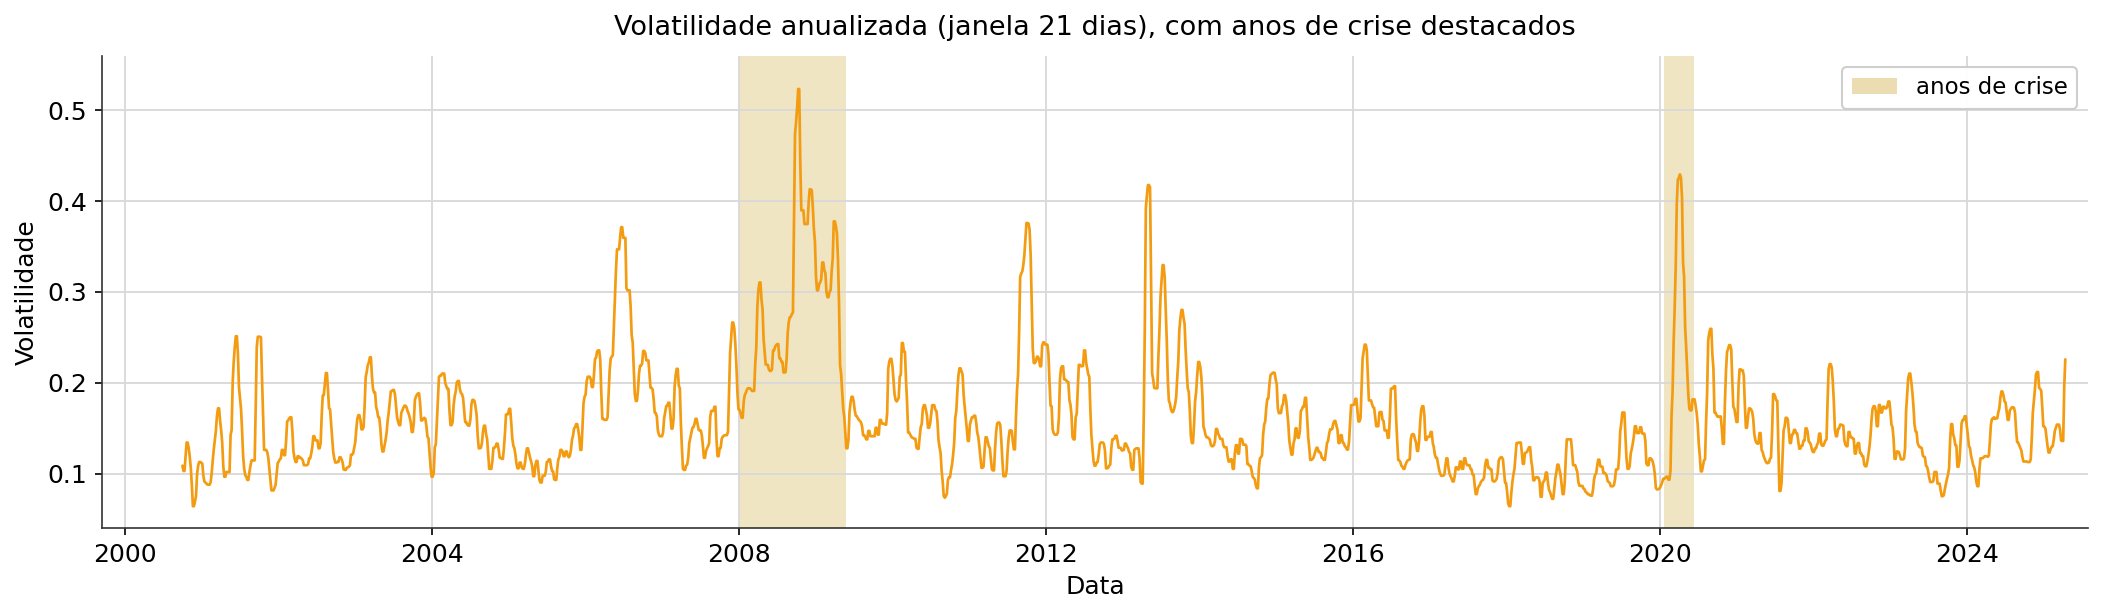
\includegraphics[width=0.9\linewidth]{figs/volatilidade.png}
        \caption{Volatilidade anualizada com janela móvel de 21 dias.}
    \end{figure}

    \vspace{0.2cm}
    \simplebox{As crises de \textbf{2008} e \textbf{2020} concentram picos de volatilidade, evidenciando \emph{volatility clustering}.}
\end{frame}

%% ---------------------------------------------------------------------------
\section{Modelos e Métricas}
\subsection{Os Modelos}

\begin{frame}{Os modelos: do mais simples ao mais complexo}
    \begin{figure}
        \centering
        \makebox[\linewidth][c]{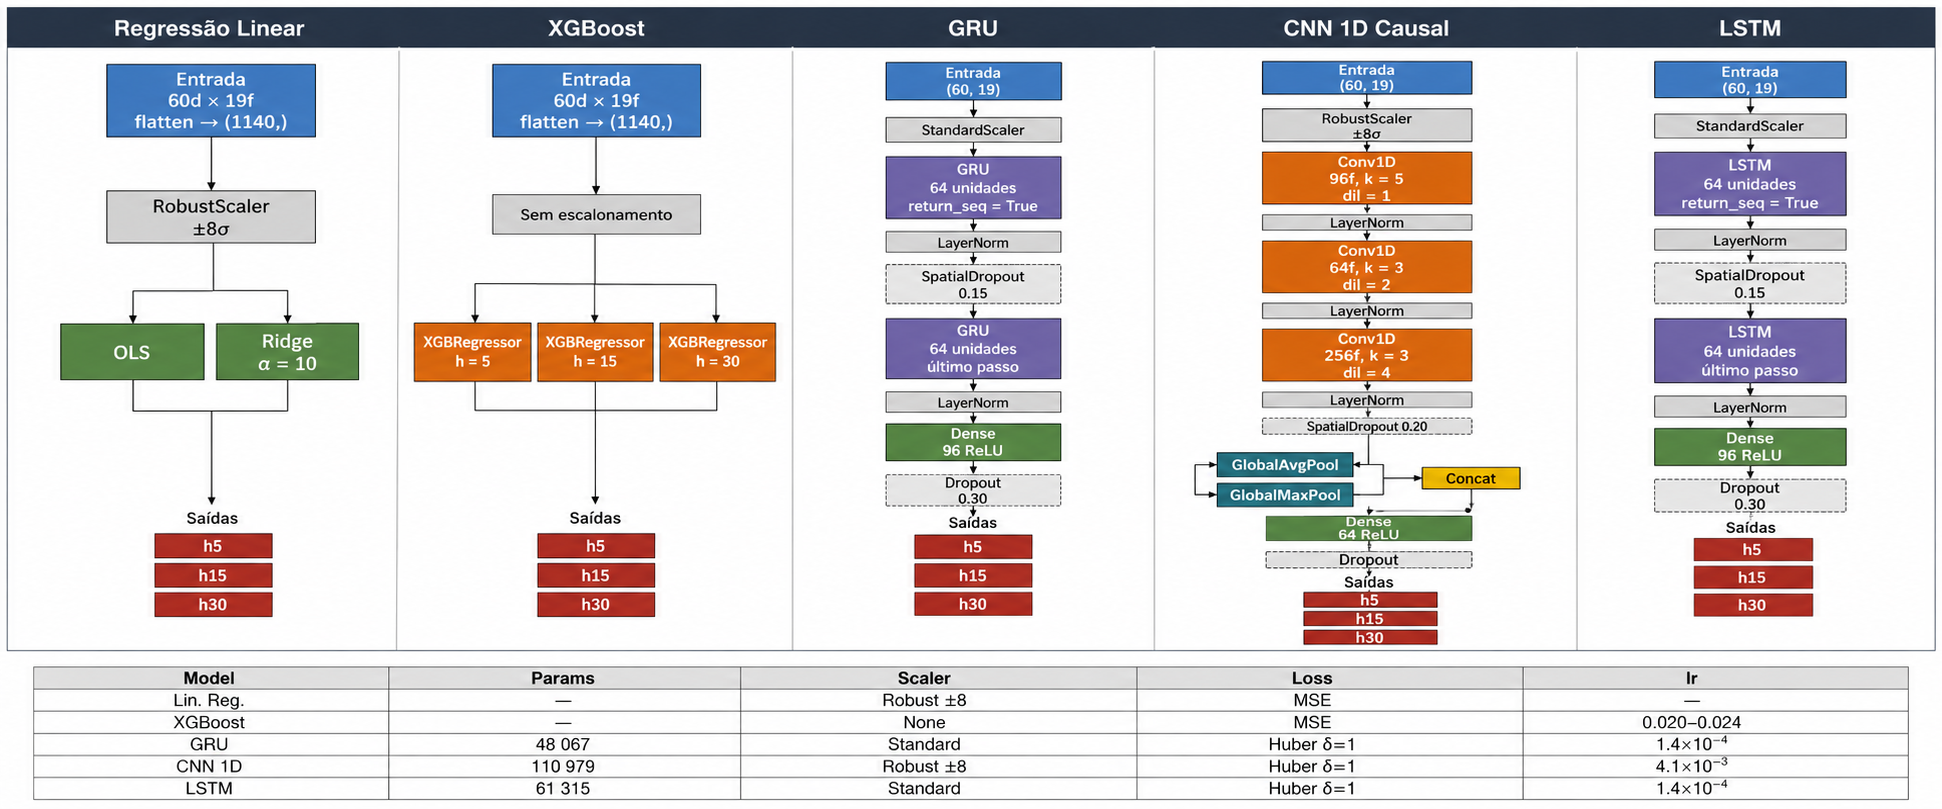
\includegraphics[width=1.14\linewidth]{figs/all_models_overview.png}}
        \caption{Visão geral dos modelos avaliados, do mais simples ao mais complexo.}
    \end{figure}
\end{frame}

%% ---------------------------------------------------------------------------
\begin{frame}{Modelos de referência}
    \begin{figure}
        \centering
        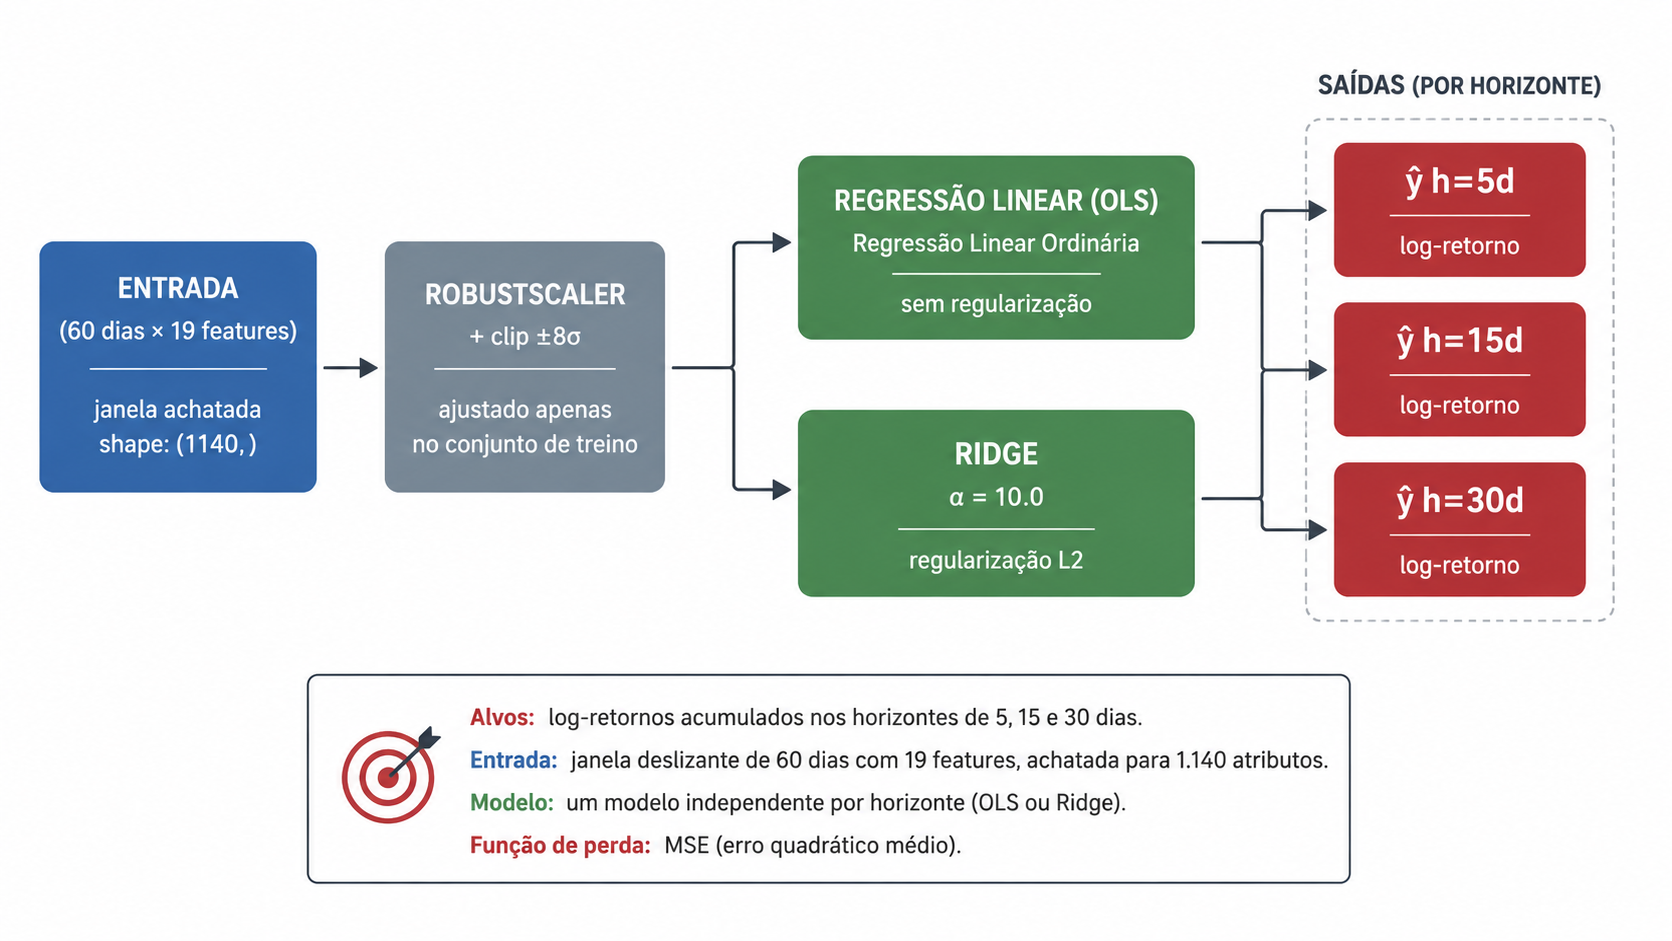
\includegraphics[width=0.95\linewidth]{figs/baseline_overview.png}
        \caption{Modelos de referência: \emph{random walk} e regressão linear.}
    \end{figure}
\end{frame}

%% ---------------------------------------------------------------------------
\begin{frame}{Modelos de referência}
    \begin{block}{Random walk}
        Piso absoluto: a previsão para $t+h$ é simplesmente o preço atual $P_t$.
    \end{block}

    \vspace{0.2cm}

    \begin{block}{Regressão linear}
        \begin{itemize}
            \item baseline treinável mais simples;
            \item usa a mesma janela temporal dos demais modelos;
            \item a janela $60 \times 19$ é achatada em \textbf{1140 regressores}.
        \end{itemize}
    \end{block}

    \vspace{0.2cm}
    \simplebox{Se modelos mais sofisticados não superarem essas referências, a complexidade extra não se justifica.}
\end{frame}

%% ---------------------------------------------------------------------------
\begin{frame}{XGBoost}
    \begin{figure}
        \centering
        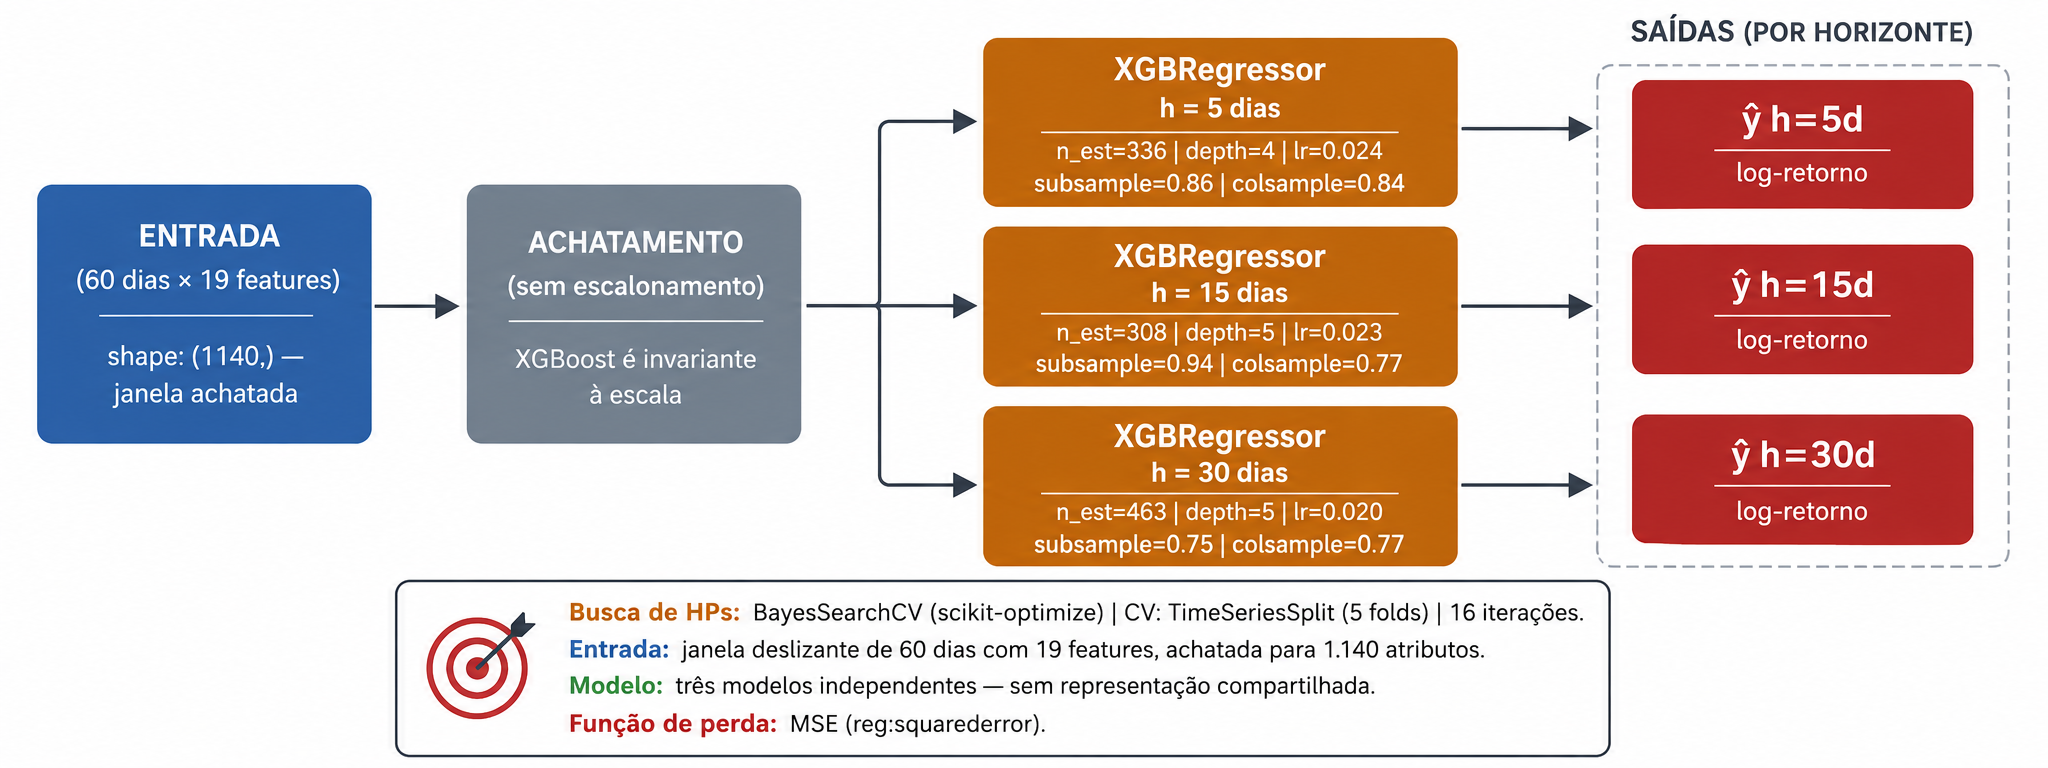
\includegraphics[width=0.95\linewidth]{figs/xgboost_overview.png}
        \caption{Visão geral do modelo XGBoost.}
    \end{figure}
\end{frame}

%% ---------------------------------------------------------------------------
\begin{frame}{XGBoost}
    \begin{itemize}
        \item Primeiro modelo não linear forte do trabalho.
        \item Implementado como \emph{gradient boosting} de árvores \cite{chen2016xgboost}.
        \item Treinado \textbf{separadamente por horizonte} ($h=5,15,30$).
        \item Hiperparâmetros ajustados com \textbf{otimização bayesiana} e validação cruzada temporal.
        \item Funciona bem com dados tabulares e interações não lineares entre atributos.
    \end{itemize}

    \vspace{0.3cm}
    \simplebox{\textbf{Intuição:} cada árvore corrige parte do erro das anteriores, acumulando um modelo mais expressivo que a regressão linear.}
\end{frame}

%% ---------------------------------------------------------------------------
\begin{frame}{GRU}
    \begin{figure}
        \centering
        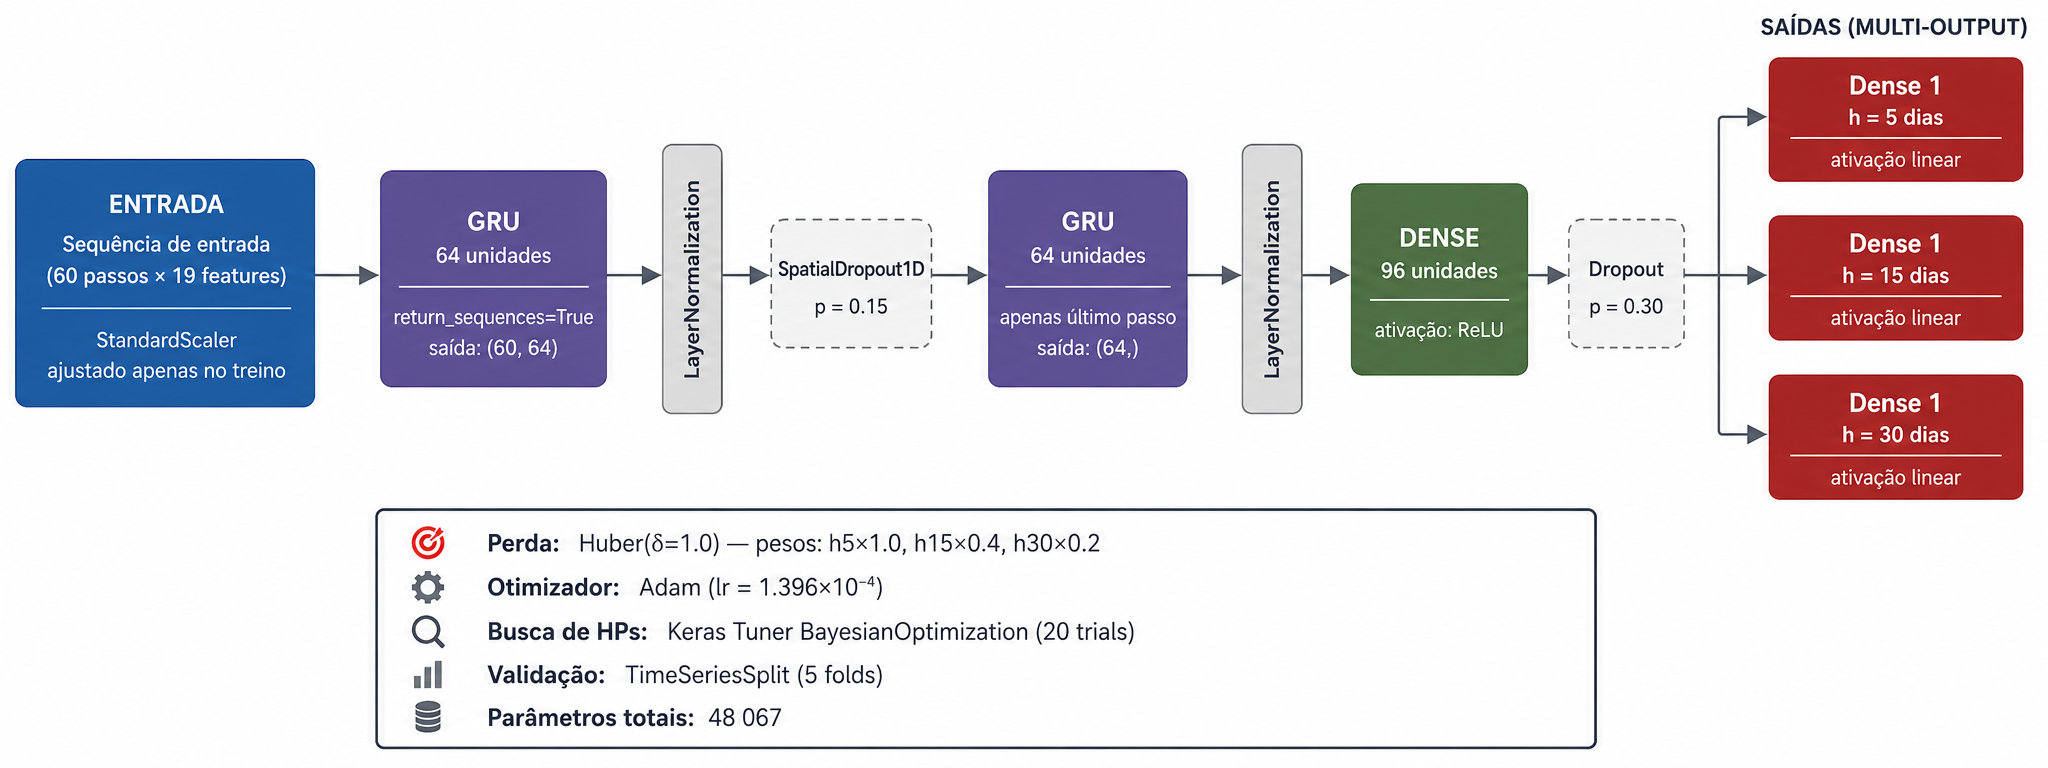
\includegraphics[width=0.95\linewidth]{figs/gru_overview.png}
        \caption{Visão geral do modelo GRU.}
    \end{figure}
\end{frame}

%% ---------------------------------------------------------------------------
\begin{frame}{LSTM}
    \begin{figure}
        \centering
        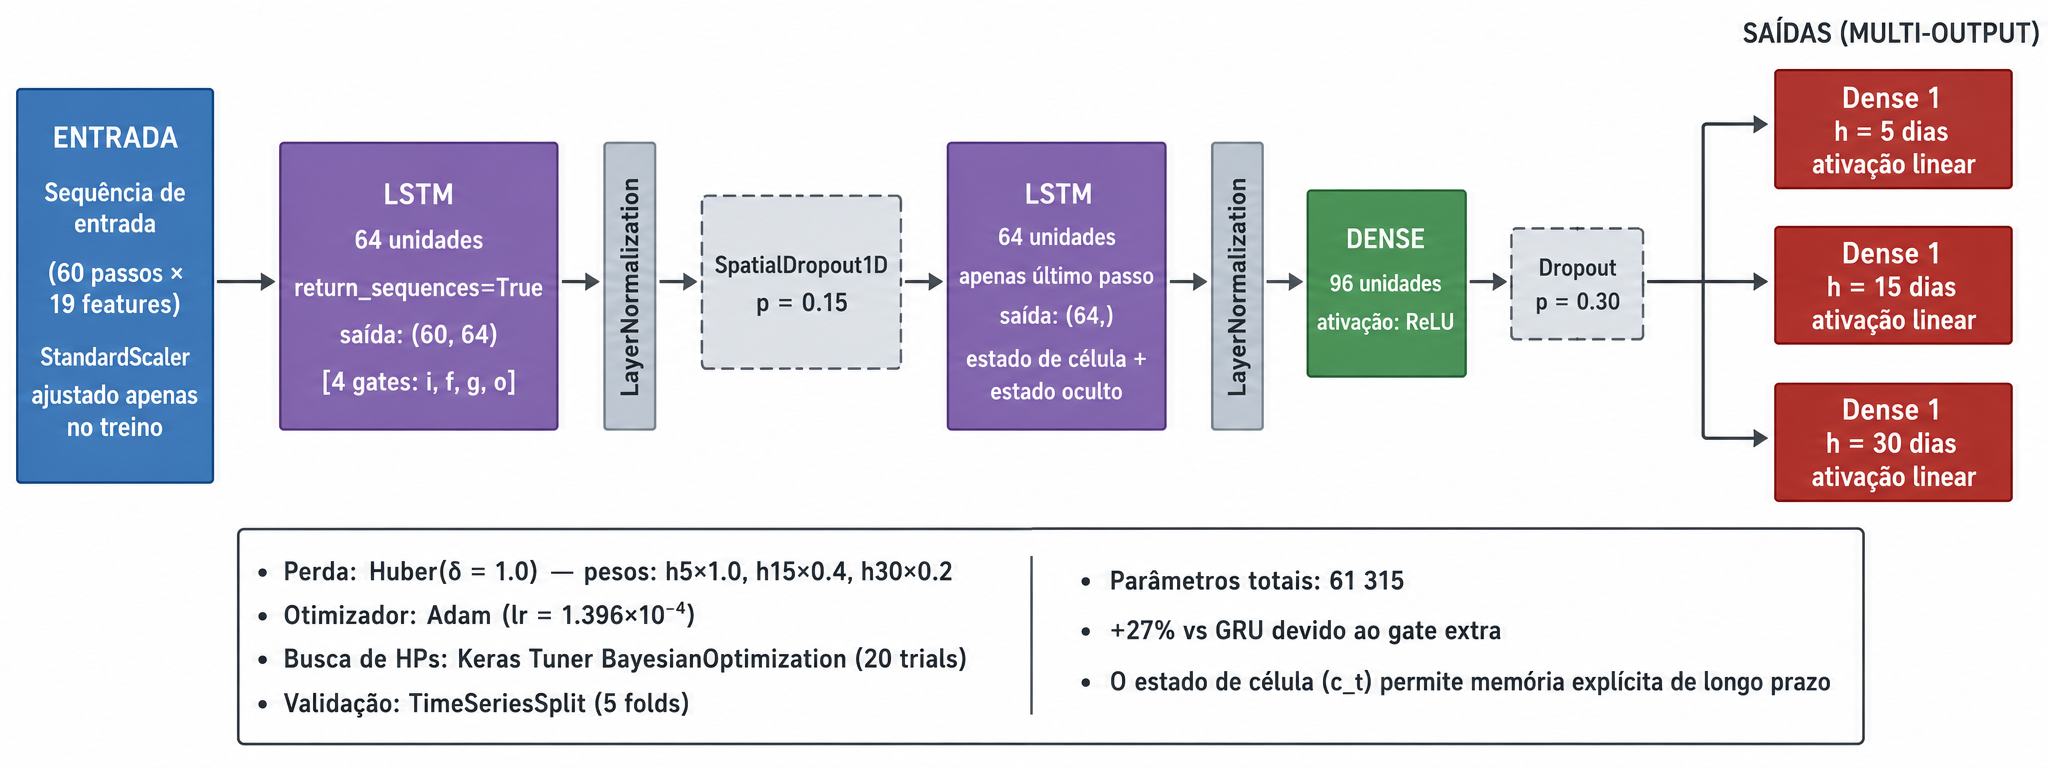
\includegraphics[width=0.95\linewidth]{figs/lstm_overview.png}
        \caption{Visão geral do modelo LSTM.}
    \end{figure}
\end{frame}

%% ---------------------------------------------------------------------------
\begin{frame}{GRU e LSTM}
    \begin{itemize}
        \item São modelos \textbf{recorrentes}: processam a janela de 60 dias passo a passo.
        \item Capturam dependências temporais de forma explícita.
        \item No trabalho, GRU e LSTM compartilham a mesma ideia de arquitetura:
        \begin{itemize}
            \item duas camadas recorrentes;
            \item normalização e \emph{dropout};
            \item \textbf{3 cabeças de saída} multitarefa para $h=5,15,30$.
        \end{itemize}
        \item A LSTM é mais expressiva; a GRU é mais enxuta em número de parâmetros.
    \end{itemize}
\end{frame}

%% ---------------------------------------------------------------------------
\begin{frame}{CNN 1D causal}
    \begin{figure}
        \centering
        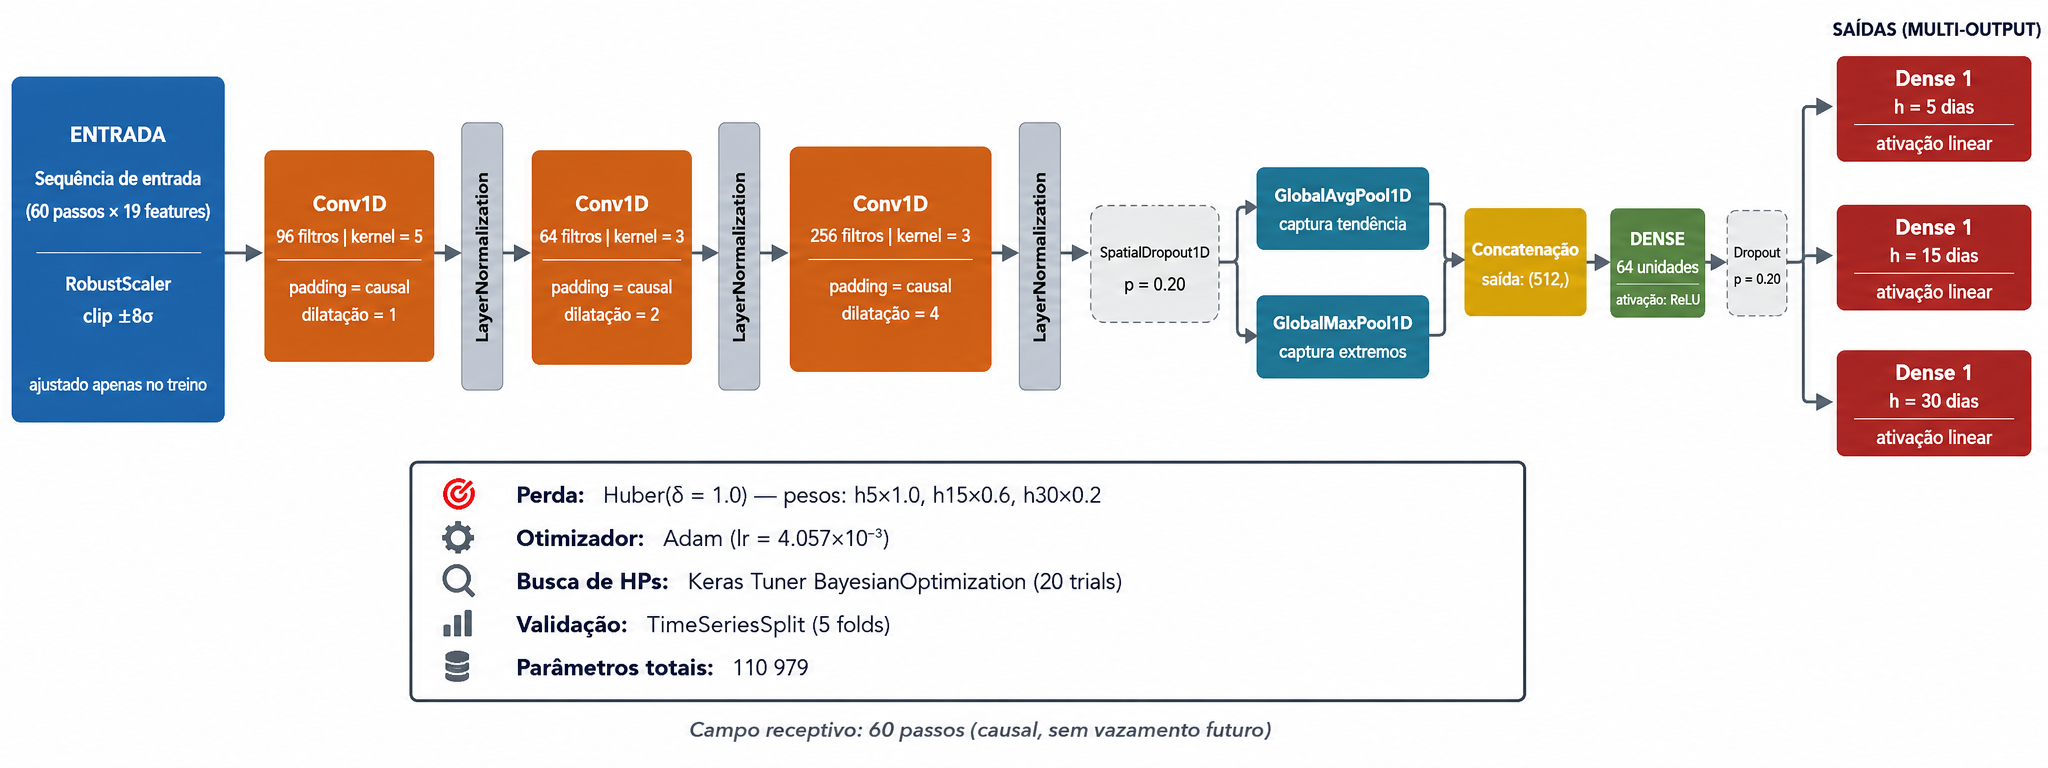
\includegraphics[width=0.95\linewidth]{figs/cnn_1d_casual_overview.png}
        \caption{Visão geral da CNN 1D causal com dilatação.}
    \end{figure}
\end{frame}

%% ---------------------------------------------------------------------------
\begin{frame}{CNN 1D causal: modelo champion}
    \begin{itemize}
        \item Modelo principal do trabalho.
        \item Usa \textbf{convoluções causais} com dilatação crescente: $1 \rightarrow 2 \rightarrow 4$.
        \item Essa dilatação amplia o campo receptivo e permite cobrir 60 dias com poucas camadas.
        \item A saída combina \emph{pooling} médio e máximo global antes das cabeças multitarefa.
        \item Tamanho: \textbf{110.979 parâmetros treináveis}.
    \end{itemize}

    \vspace{0.3cm}
    \successbox{\textbf{Intuição:} a CNN enxerga padrões locais e de médio alcance sem precisar percorrer a sequência inteira passo a passo como uma RNN.}
\end{frame}

%% ---------------------------------------------------------------------------
\begin{frame}{Configuração final dos modelos neurais}
    \scriptsize
    \begin{table}
    \centering
    \caption{Configuração final dos modelos neurais avaliados.}
    \begin{tabular}{p{0.33\linewidth} p{0.28\linewidth} p{0.28\linewidth}}
        \toprule
        \textbf{Hiperparâmetro} & \textbf{CNN 1D} & \textbf{GRU / LSTM} \\
        \midrule
        Camadas extratoras & 3 $\times$ Conv1D causal & 2 $\times$ recorrente (64) \\
        Filtros / unidades & 96, 64, 256 & 64, 64 \\
        Dilatação / kernel & $1{\to}2{\to}4$ / 5,3,3 & --- \\
        \emph{Spatial Dropout} & 0{,}20 & 0{,}15 \\
        Densa + \emph{Dropout} & 64 / 0{,}20 & 64 / 0{,}25 \\
        Taxa de aprendizado & $4{,}1\times10^{-3}$ & $1{,}0\times10^{-3}$ \\
        Pesos da perda & 1{,}0 / 0{,}6 / 0{,}2 & 1{,}0 / 0{,}7 / 0{,}5 \\
        Épocas / \emph{batch} & 120 / 64 & 120 / 64 \\
        \emph{Early stopping} & paciência 15 & paciência 15 \\
        Parâmetros treináveis & 110.979 & $\approx 60$--$80$ mil \\
        \bottomrule
    \end{tabular}
    \end{table}
\end{frame}

%% ---------------------------------------------------------------------------
\begin{frame}{Extensão: CNN por quantis}
    \begin{itemize}
        \item Extensão do modelo principal para prever \textbf{quantis} em vez de um único valor.
        \item Saídas: \textbf{$q10$, $q50$, $q90$} para cada horizonte.
        \item Função de perda: \textbf{pinball loss}, adequada para regressão quantílica \cite{koenkerbassett1978}.
        \item Aplicação principal: validação \emph{walk-forward} com \textbf{intervalos de incerteza}.
    \end{itemize}

    \vspace{0.3cm}
    \simplebox{\textbf{Ganho prático:} em vez de uma estimativa pontual aparentemente precisa, o modelo comunica uma faixa plausível de preço futuro (\(p10\)–\(p90\)).}
\end{frame}

%% ---------------------------------------------------------------------------
\subsection{Métricas}

\begin{frame}{Métricas}
    \begin{itemize}
        \item A avaliação principal usa duas métricas centrais:
        \begin{itemize}
            \item \textbf{MAE/MAE\(_{naive}\)}: compara o erro do modelo com o erro do \emph{random walk};
            \item \textbf{acurácia direcional}: mede quantas vezes o modelo acertou o sinal do retorno.
        \end{itemize}
        \item Essas são métricas \textbf{honestas} porque respondem à pergunta prática: o modelo realmente superou uma referência ingênua?
        \item Valores de \textbf{MAE/MAE\(_{naive}\) abaixo de 1} indicam ganho real sobre o baseline.
    \end{itemize}
\end{frame}

%% ---------------------------------------------------------------------------
\begin{frame}{Por que essas métricas são mais honestas?}
    \begin{columns}
        \begin{column}{0.48\textwidth}
            \begin{exampleblock}{MAE/MAE\(_{naive}\)}
                \centering
                \Large \textbf{0,95}

                \vspace{0.2cm}
                \normalsize erro 5\% menor que o\\ \emph{random walk}
            \end{exampleblock}
        \end{column}
        \begin{column}{0.48\textwidth}
            \begin{block}{Acurácia direcional}
                \centering
                \Large \textbf{62\%}

                \vspace{0.2cm}
                \normalsize acerto no sentido\\ da variação
            \end{block}
        \end{column}
    \end{columns}

    \vspace{0.4cm}
    \simplebox{\textbf{Ideia:} não basta errar pouco em dólares; é preciso bater a previsão ingênua e acertar a direção do movimento.}
\end{frame}

%% ---------------------------------------------------------------------------
\begin{frame}{Alerta: \(R^2\) no preço pode enganar}
    \begin{columns}
        \begin{column}{0.48\textwidth}
            \begin{exampleblock}{Parece ótimo}
                \centering
                \Large \textbf{\(R^2 = 0{,}98\)}

                \vspace{0.3cm}
                \normalsize na escala de preço
            \end{exampleblock}
        \end{column}
        \begin{column}{0.48\textwidth}
            \begin{alertblock}{Mas pode empatar}
                \centering
                \Large \textbf{MAE/naive \(= 1{,}0\)}

                \vspace{0.3cm}
                \normalsize mesmo desempenho do\\ \emph{random walk}
            \end{alertblock}
        \end{column}
    \end{columns}

    \vspace{0.4cm}
    \alertbox{\textbf{Gancho para a discussão:} um \(R^2\) altíssimo no preço pode ser só reflexo da tendência da série, sem ganho preditivo real.}
\end{frame}

%% ---------------------------------------------------------------------------
\section{Resultados e Discussão}
\subsection{Resultados}

\begin{frame}{Split único: três achados principais}
    \begin{itemize}
        \item A \textbf{regressão linear não bate} o \emph{random walk} de forma consistente.
        \item \textbf{CNN 1D} e \textbf{XGBoost} superam o baseline ingênuo em \textbf{todos os horizontes}.
        \item O ganho fica mais claro em horizontes longos: em \(h=30\), ambos chegam a cerca de \textbf{62\%} de acurácia direcional.
    \end{itemize}

    \vspace{0.3cm}
    \simplebox{\textbf{Leitura:} no recorte de teste único, há sinal útil, mas ele é pequeno e aparece mais nitidamente quando o horizonte aumenta.}
\end{frame}

%% ---------------------------------------------------------------------------
\begin{frame}{Desempenho no split único}
    \scriptsize
    \begin{table}
    \centering
    \caption{Desempenho dos modelos no split único cronológico, por horizonte.}
    \begin{tabular}{llccccc}
        \toprule
        \(h\) & \textbf{Modelo} & \textbf{MAE} & \textbf{RMSE} & \textbf{MAPE (\%)} & \textbf{Dir.\ (\%)} & \textbf{MAE/naive} \\
        \midrule
        \multirow{5}{*}{5}
          & Regressão Linear & 38{,}23 & 48{,}20 & 1{,}82 & 52{,}5 & 1{,}160 \\
          & XGBoost          & 32{,}53 & 41{,}62 & 1{,}56 & 56{,}5 & 0{,}987 \\
          & GRU              & 32{,}65 & 41{,}77 & 1{,}57 & 53{,}4 & 0{,}990 \\
          & LSTM             & 32{,}62 & 41{,}50 & 1{,}57 & 53{,}3 & 0{,}989 \\
          & \textbf{CNN 1D}  & 32{,}39 & 41{,}42 & 1{,}56 & 57{,}4 & \textbf{0{,}983} \\
        \midrule
        \multirow{5}{*}{15}
          & Regressão Linear & 63{,}87 & 80{,}22 & 3{,}05 & 55{,}0 & 1{,}068 \\
          & XGBoost          & 58{,}26 & 73{,}11 & 2{,}78 & 58{,}9 & 0{,}974 \\
          & GRU              & 59{,}56 & 74{,}36 & 2{,}84 & 56{,}5 & 0{,}996 \\
          & LSTM             & 58{,}48 & 73{,}23 & 2{,}78 & 54{,}8 & 0{,}978 \\
          & \textbf{CNN 1D}  & 58{,}08 & 72{,}68 & 2{,}77 & 58{,}9 & \textbf{0{,}971} \\
        \midrule
        \multirow{5}{*}{30}
          & Regressão Linear & 87{,}66 & 109{,}09 & 4{,}16 & 58{,}4 & 1{,}002 \\
          & \textbf{XGBoost} & 83{,}16 & 101{,}45 & 3{,}89 & 62{,}0 & \textbf{0{,}951} \\
          & GRU              & 85{,}00 & 103{,}70 & 3{,}97 & 58{,}7 & 0{,}972 \\
          & LSTM             & 85{,}77 & 103{,}49 & 4{,}02 & 57{,}6 & 0{,}980 \\
          & CNN 1D           & 83{,}43 & 102{,}38 & 3{,}92 & 62{,}0 & 0{,}954 \\
        \bottomrule
    \end{tabular}
    \end{table}
\end{frame}

%% ---------------------------------------------------------------------------
\begin{frame}{Curvas de aprendizado da CNN}
    \begin{figure}
        \centering
        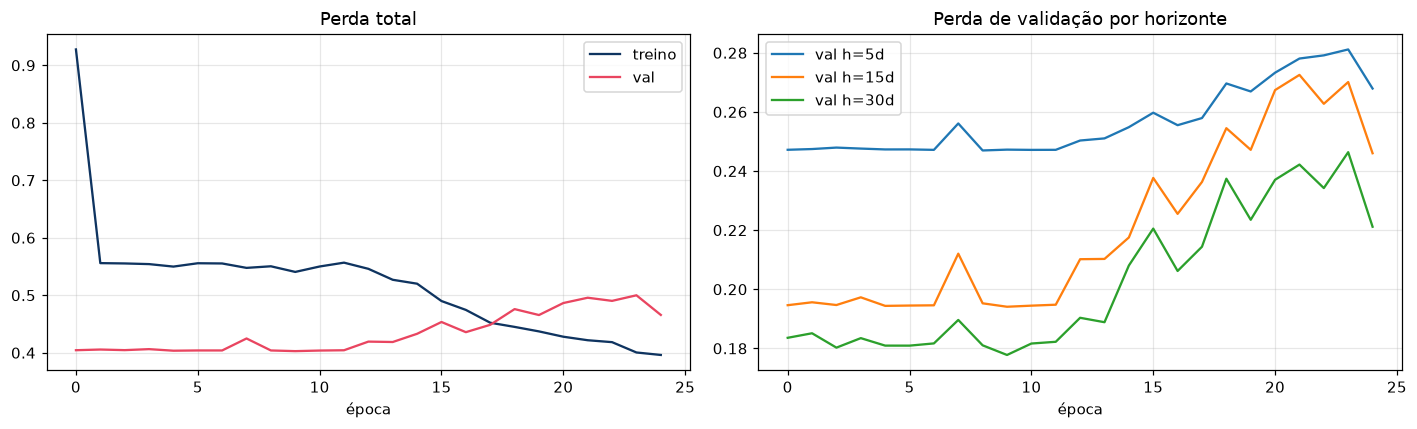
\includegraphics[width=\linewidth]{figs/cnn_curvas_treino.png}
        \caption{Curvas de treino e validação da CNN principal.}
    \end{figure}
\end{frame}

%% ---------------------------------------------------------------------------
{\logo{}
\begin{frame}{Preço real vs. previsto}
    \begin{figure}
        \centering
        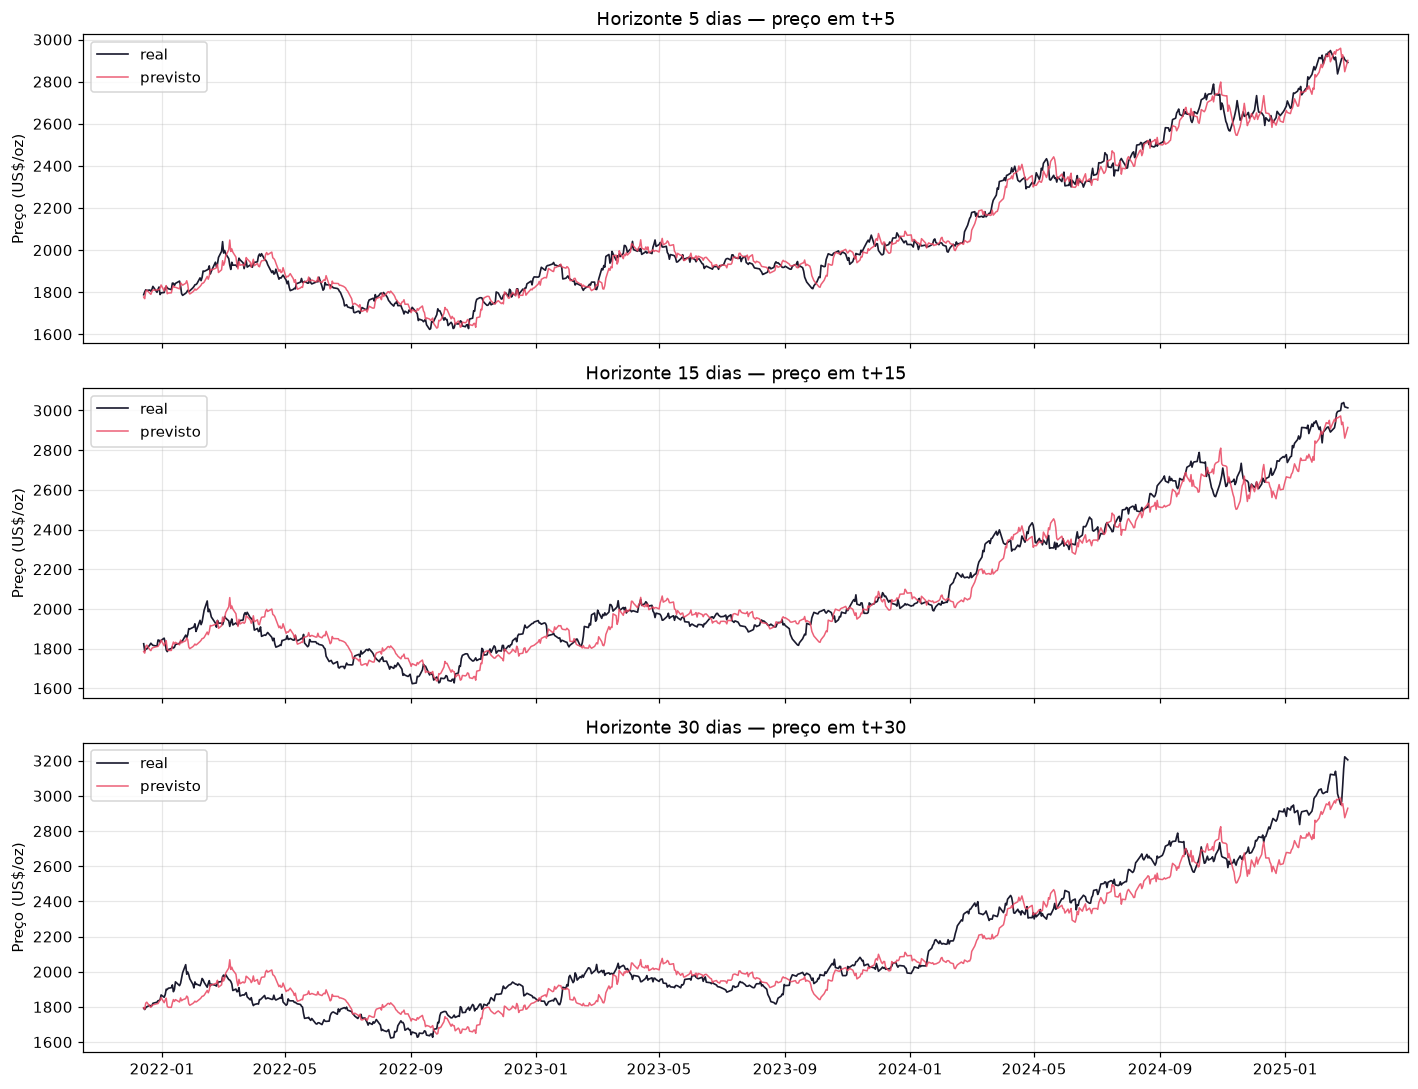
\includegraphics[width=0.85\linewidth]{figs/cnn_pred_vs_real.png}
        \caption{Preço real e previsto pela CNN em \(h=5\), \(h=15\) e \(h=30\).}
    \end{figure}

    \vspace{0.2cm}
    \simplebox{A CNN acompanha a tendência, mas \textbf{suaviza os choques} e introduz mais atraso à medida que o horizonte cresce.}
\end{frame}
}

%% ---------------------------------------------------------------------------
\begin{frame}{E se o split de teste só deu sorte?}
    \centering
    \Huge \textbf{E se o split de teste só deu sorte?}
\end{frame}

%% ---------------------------------------------------------------------------
\begin{frame}{Walk-forward: a virada honesta}
    \begin{itemize}
        \item Quando avaliamos com \emph{walk-forward}, o quadro fica bem menos otimista.
        \item A vantagem média sobre o \emph{random walk} fica \textbf{próxima de 1,0}.
        \item O desvio entre \emph{folds} é alto, principalmente em \(h=30\).
        \item Ou seja: o ganho existe em alguns regimes, mas \textbf{não é estável} ao longo do tempo.
    \end{itemize}

    \vspace{0.3cm}
    \alertbox{\textbf{Leitura correta:} o split único mostrava um caso favorável; o walk-forward revela a robustez real do método.}
\end{frame}

%% ---------------------------------------------------------------------------
\begin{frame}{Validação walk-forward}
    \scriptsize
    \begin{table}
    \centering
    \caption{Desempenho médio \(\pm\) desvio-padrão dos modelos neurais na validação walk-forward.}
    \begin{tabular}{llcc}
        \toprule
        \textbf{Modelo} & \(h\) & \textbf{Dir.\ (\%)} & \textbf{MAE/naive} \\
        \midrule
        \multirow{3}{*}{CNN 1D}
          & 5  & \textbf{55{,}3 \(\pm\) 5{,}7}  & \textbf{0{,}995 \(\pm\) 0{,}024} \\
          & 15 & 54{,}8 \(\pm\) 8{,}4           & \textbf{1{,}006 \(\pm\) 0{,}055} \\
          & 30 & 54{,}8 \(\pm\) 13{,}9          & \textbf{1{,}037 \(\pm\) 0{,}138} \\
        \midrule
        \multirow{3}{*}{GRU}
          & 5  & 51{,}5 \(\pm\) 2{,}0           & 1{,}042 \(\pm\) 0{,}038 \\
          & 15 & 53{,}9 \(\pm\) 6{,}6           & 1{,}047 \(\pm\) 0{,}067 \\
          & 30 & \textbf{58{,}1 \(\pm\) 12{,}1} & 1{,}074 \(\pm\) 0{,}225 \\
        \midrule
        \multirow{3}{*}{LSTM}
          & 5  & 51{,}4 \(\pm\) 4{,}0           & 1{,}048 \(\pm\) 0{,}047 \\
          & 15 & \textbf{55{,}1 \(\pm\) 4{,}5}  & 1{,}049 \(\pm\) 0{,}068 \\
          & 30 & 55{,}9 \(\pm\) 10{,}7          & 1{,}075 \(\pm\) 0{,}193 \\
        \bottomrule
    \end{tabular}
    \end{table}
\end{frame}

%% ---------------------------------------------------------------------------
\begin{frame}{Boxplots no walk-forward}
    \begin{figure}
        \centering
        \makebox[\linewidth][c]{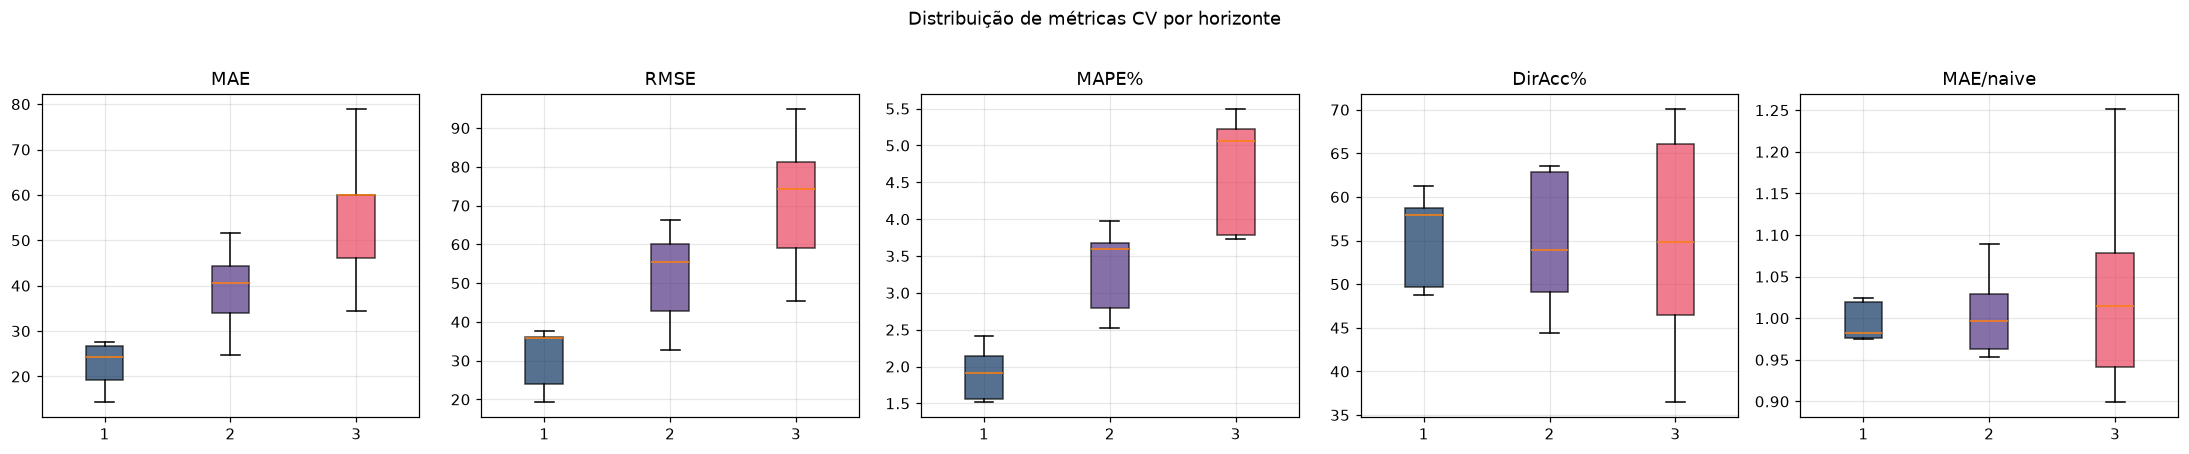
\includegraphics[width=1.1\linewidth]{figs/cnn_cv_boxplot.png}}
        \caption{Distribuição das métricas da CNN entre folds no walk-forward.}
    \end{figure}
\end{frame}

%% ---------------------------------------------------------------------------
\begin{frame}{Por que isso acontece?}
    \begin{itemize}
        \item O desempenho depende fortemente do \textbf{regime de mercado}.
        \item Em anos de tendência forte, os modelos conseguem capturar direção.
        \item Em mercados laterais e ruidosos, o sinal praticamente desaparece.
    \end{itemize}

    \vspace{0.3cm}
    \simplebox{\textbf{Frase-chave:} os modelos capturam tendência quando ela existe, mas não ``criam'' sinal onde ele não existe.}
\end{frame}

%% ---------------------------------------------------------------------------
\begin{frame}{Desempenho por ano em \(h=30\)}
    \begin{figure}
        \centering
        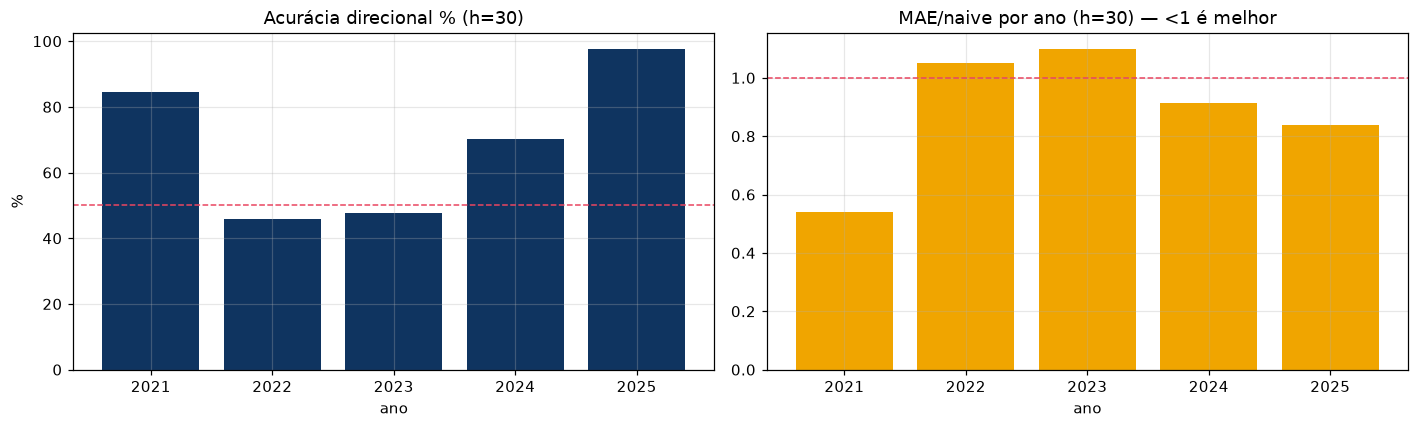
\includegraphics[width=0.93\linewidth]{figs/cnn_anual_h30.png}
        \caption{Acurácia direcional e MAE/naive por ano calendário para a CNN em \(h=30\).}
    \end{figure}
\end{frame}

%% ---------------------------------------------------------------------------
\begin{frame}{Leitura por regime}
    \begin{itemize}
        \item Em anos de tendência, como \textbf{2021}, \textbf{2024} e \textbf{2025}, a acurácia direcional passa de \textbf{80\%} e o MAE/naive cai abaixo de \textbf{0,85}.
        \item Em mercados laterais, como \textbf{2022} e \textbf{2023}, a acurácia cai para algo como \textbf{46--48\%}, isto é, \textbf{pior que o acaso}.
        \item Isso explica por que o split único parecia forte, mas o walk-forward mostrou instabilidade.
    \end{itemize}
\end{frame}

%% ---------------------------------------------------------------------------
\subsection{Discussão}

\begin{frame}{\(R^2\) alto pode ser ilusão}
    \begin{figure}
        \centering
        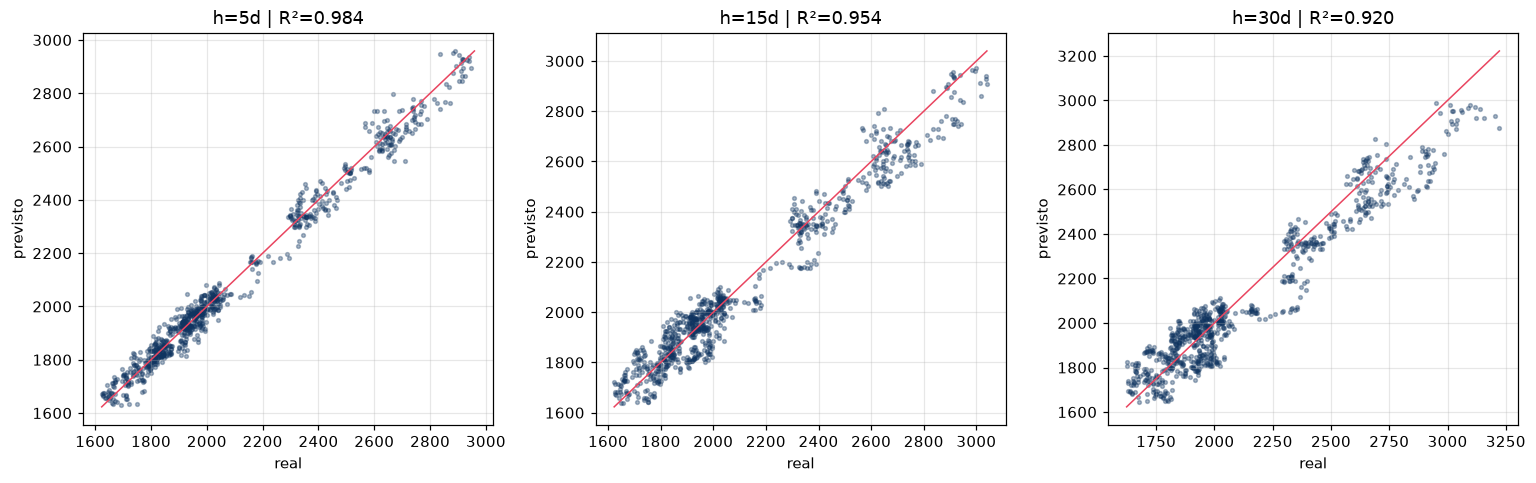
\includegraphics[width=0.96\linewidth]{figs/cnn_scatter.png}
        \caption{Dispersão entre preço previsto e preço real no teste para a CNN.}
    \end{figure}

    \vspace{0.2cm}
    \alertbox{\textbf{Ponto central:} mesmo com \(R^2\) entre 0,92 e 0,98, o ganho real sobre o \emph{random walk} pode ser apenas marginal.}
\end{frame}

%% ---------------------------------------------------------------------------
\begin{frame}{Quem foi mais estável?}
    \begin{itemize}
        \item No \emph{split} único, CNN 1D e XGBoost praticamente empatam entre os melhores.
        \item No \emph{walk-forward}, a \textbf{CNN} fica mais estável e com média mais próxima de ganho real consistente.
        \item GRU e LSTM ficam mais sensíveis à variação entre regimes.
        \item Por isso, a CNN 1D causal foi escolhida como \textbf{modelo principal} do trabalho.
    \end{itemize}
\end{frame}

%% ---------------------------------------------------------------------------
\begin{frame}{Heatmap de acurácia direcional em \(h=30\)}
    \begin{figure}
        \centering
        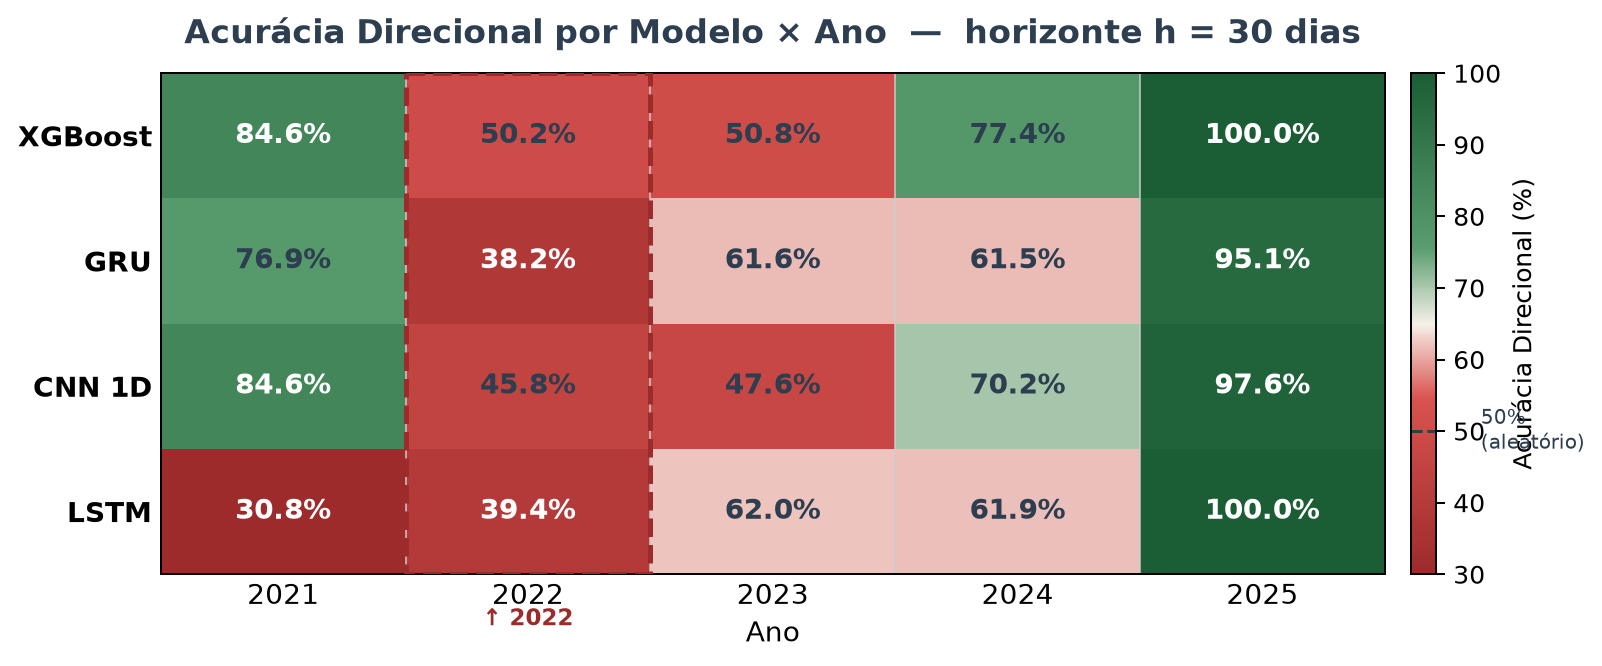
\includegraphics[width=0.94\linewidth]{figs/diracc_heatmap_h30.png}
        \caption{Acurácia direcional por modelo e por ano em \(h=30\).}
    \end{figure}
\end{frame}

%% ---------------------------------------------------------------------------
\begin{frame}{Onde os modelos falham}
    \begin{itemize}
        \item O heatmap deixa claro que \textbf{2022} e \textbf{2023} são anos difíceis para todos os modelos.
        \item Esses períodos são mais laterais e ruidosos, com pouco sinal direcional persistente.
        \item O índice de medo por léxico ajuda pouco: a informação textual ainda está subexplorada.
        \item Isso reforça a leitura final do trabalho: \textbf{os modelos capturam tendência quando ela existe, mas não ``criam'' sinal}. 
    \end{itemize}
\end{frame}

%% ---------------------------------------------------------------------------
\section{Conclusão}

\begin{frame}{Conclusão}
    \begin{itemize}
        \item \textbf{Primeiro achado:} reformular o problema em \textbf{log-retorno} foi essencial para torná-lo estatisticamente bem posto.
        \item \textbf{Segundo achado:} no \emph{split} recente, \textbf{CNN 1D} e \textbf{XGBoost} superam o \emph{random walk}.
        \item \textbf{Terceiro achado:} sob validação \emph{walk-forward}, esse ganho fica \textbf{pequeno} e \textbf{dependente do regime}.
    \end{itemize}

    \vspace{0.3cm}
    \simplebox{\textbf{Mensagem final:} o trabalho mostra que existe sinal preditivo marginal, mas ele é frágil e não sobrevive de forma uniforme a todos os cenários de mercado.}
\end{frame}

%% ---------------------------------------------------------------------------
\begin{frame}{Limitações}
    \begin{itemize}
        \item O sinal direcional é intrinsecamente \textbf{fraco}.
        \item O estudo foi feito sobre \textbf{um único ativo} e um \textbf{único período histórico}.
        \item O componente textual foi tratado de forma \textbf{rudimentar}, com um léxico simples de medo.
        \item Portanto, os resultados não devem ser lidos como solução geral para previsão financeira.
    \end{itemize}
\end{frame}

%% ---------------------------------------------------------------------------
\begin{frame}{Trabalhos futuros}
    \begin{itemize}
        \item Substituir o léxico de medo por \textbf{embeddings} ou modelos de \textbf{sentimento financeiro}.
        \item Incorporar variáveis macroeconômicas causais, como \textbf{juros reais}, \textbf{dólar} e \textbf{outros metais}.
        \item Avaliar arquiteturas com atenção, como o \textbf{Temporal Fusion Transformer}.
        \item Fazer \textbf{calibração formal} dos intervalos previstos pela CNN por quantis.
    \end{itemize}

    \vspace{0.3cm}
    \successbox{O caminho promissor não é só aumentar a complexidade do modelo, mas enriquecer causalmente a informação e medir melhor a incerteza.}
\end{frame}

%% ---------------------------------------------------------------------------
% Reference frames
\begin{frame}[allowframebreaks]
    \frametitle{Referências}
    \printbibliography
\end{frame}

%% ---------------------------------------------------------------------------
% Final frame
\begin{frame}{}
    \centering
    \huge{\textbf{\example{Obrigado(a) pela Atenção!}}}
    
    \vspace{1cm}
    
    \Large{\textbf{Contato:}}
    \newline
    \vspace*{0.5cm}
    \large{\email{\{paulinofilho, ivinalorena, gabrielmendes01, joseedsouza\}@alu.ufc.br}}
\end{frame}

\end{document}
